\documentclass[10pt]{article}  

%%%%%%%% PREÁMBULO %%%%%%%%%%%%
\title{Plantilla para prácticas de UGR}
\usepackage[spanish]{babel} %Indica que escribiermos en español
\usepackage[utf8]{inputenc} %Indica qué codificación se está usando ISO-8859-1(latin1)  o utf8  
\usepackage{amsmath} % Comandos extras para matemáticas (cajas para ecuaciones,
% etc)
\usepackage{amssymb} % Simbolos matematicos (por lo tanto)
\usepackage{graphicx} % Incluir imágenes en LaTeX
\usepackage{color} % Para colorear texto
\usepackage{subfigure} % subfiguras
\usepackage{float} %Podemos usar el especificador [H] en las figuras para que se
% queden donde queramos
\usepackage{capt-of} % Permite usar etiquetas fuera de elementos flotantes
% (etiquetas de figuras)
\usepackage{sidecap} % Para poner el texto de las imágenes al lado
	\sidecaptionvpos{figure}{c} % Para que el texto se alinie al centro vertical
\usepackage{caption} % Para poder quitar numeracion de figuras
\usepackage{commath} % funcionalidades extras para diferenciales, integrales,
% etc (\od, \dif, etc)
\usepackage{cancel} % para cancelar expresiones (\cancelto{0}{x})

\graphicspath{{/Users/jesusgarciamanday/Desktop/Master/CC-II/Practicas/Practica3/p3/Imagenes/}}

\usepackage{anysize} 					% Para personalizar el ancho de  los márgenes
\marginsize{2cm}{2cm}{2cm}{2cm} % Izquierda, derecha, arriba, abajo

\usepackage{appendix}
\renewcommand{\appendixname}{Apéndices}
\renewcommand{\appendixtocname}{Apéndices}
\renewcommand{\appendixpagename}{Apéndices} 

% Para que las referencias sean hipervínculos a las figuras o ecuaciones y
% aparezcan en color
\usepackage[colorlinks=true,plainpages=true,citecolor=blue,linkcolor=blue]{hyperref}
%\usepackage{hyperref} 
% Para agregar encabezado y pie de página
\usepackage{fancyhdr} 
\pagestyle{fancy}
\fancyhf{}
\fancyhead[L]{\footnotesize UGR} %encabezado izquierda
\fancyhead[R]{\footnotesize CCIA}   % dereecha
\fancyfoot[R]{\footnotesize Pr\'actica 2 - Docker }  % Pie derecha
\fancyfoot[C]{\thepage}  % centro
\fancyfoot[L]{\footnotesize Master en Ingenier\'ia Inform\'atica }  %izquierda
\renewcommand{\footrulewidth}{0.4pt}


\usepackage{listings} % Para usar código fuente
\definecolor{dkgreen}{rgb}{0,0.6,0} % Definimos colores para usar en el código
\definecolor{gray}{rgb}{0.5,0.5,0.5} 
% configuración para el lenguaje que queramos utilizar
\lstset{language=Matlab,
   keywords={break,case,catch,continue,else,elseif,end,for,function,
      global,if,otherwise,persistent,return,switch,try,while},
   basicstyle=\ttfamily,
   keywordstyle=\color{blue},
   commentstyle=\color{red},
   stringstyle=\color{dkgreen},
   numbers=left,
   numberstyle=\tiny\color{gray},
   stepnumber=1,
   numbersep=10pt,
   backgroundcolor=\color{white},
   tabsize=4,
   showspaces=false,
   showstringspaces=false}

\newcommand{\sen}{\operatorname{\sen}}	% Definimos el comando \sen para el seno
%en español

\title{Práctica 3 - Bases de Datos NoSQL}

%%%%%%%% TERMINA PREÁMBULO %%%%%%%%%%%%

\begin{document}

%%%%%%%%%%%%%%%%%%%%%%%%%%%%%%%%%% PORTADA %%%%%%%%%%%%%%%%%%%%%%%%%%%%%%%%%%%%%%%%%%%%
																					%%%
\begin{center}																		%%%
\newcommand{\HRule}{\rule{\linewidth}{0.5mm}}									%%%\left
 																					%%%
\begin{minipage}{0.48\textwidth} \begin{flushleft}
%
\includegraphics[scale = 0.63]{Imagenes/logo_upiita}
\end{flushleft}\end{minipage}
\begin{minipage}{0.48\textwidth} \begin{flushright}
%
\includegraphics[scale = 0.35]{Imagenes/IPN}
\end{flushright}\end{minipage}

													 								%%%
\vspace*{-1.5cm}								%%%
																					%%%	
\textsc{\huge Universidad de\\ \vspace{5px} Granada}\\[1.5cm]	

\textsc{\LARGE Master Profesional en Ingenier\'ia Inform\'atica }\\[1.5cm]													%%%

\begin{minipage}{0.9\textwidth} 
\begin{center}																					%%%
\textsc{\LARGE Pr\'actica 2}
\end{center}
\end{minipage}\\[0.5cm]
%%%
    																				%%%
 			\vspace*{1cm}																		%%%
																					%%%
\HRule \\[0.4cm]																	%%%
{ \huge \bfseries MongoDB}\\[0.4cm]	%%%
 																					%%%
\HRule \\[1.5cm]																	%%%
 																				%%%
																					%%%
\begin{minipage}{0.46\textwidth}													%%%
\begin{flushleft} \large															%%%
\emph{Autor:}\\	
Manuel Jes\'us Garc\'ia Manday (nickter@correo.ugr.es)\\
%%%
			%\vspace*{2cm}	
            													%%%
										 						%%%
\end{flushleft}																		%%%
\end{minipage}		
																%%%
\begin{minipage}{0.52\textwidth}		
\vspace{-0.6cm}											%%%
\begin{flushright} \large															%%%
													%%%
\end{flushright}																	%%%
\end{minipage}	
\vspace*{1cm}
%\begin{flushleft}
 	
%\end{flushleft}
%%%
 		\flushleft{\textbf{\Large Master en Ingenier\'ia Inform\'atica}	}\\																		%%%
\vspace{2cm} 																				
\begin{center}																					
{\large \today}																	%%%
 			\end{center}												  						
\end{center}							 											
																					
\newpage																		
%%%%%%%%%%%%%%%%%%%% TERMINA PORTADA %%%%%%%%%%%%%%%%%%%%%%%%%%%%%%%%

\tableofcontents 

\newpage

\section{Objetivo.}

El objetivo de esta práctica es familiarizarse con el uso de un sistema de gestión de bases de datos en entornos Big Data. Para ello haremos uso de la aplicación más conocida como es MongoDB.\\


\section{Consulta de Documentos.} 

Crear la colección pedidos sobre la que se realizarán diversas operaciones CRUD.

\subsection{Visualiza la colección pedidos y familiarízate con ella. Observa los distintos tipos de datos y sus estructuras dispares.}

 \begin{figure}[H]
	\begin{center}
 		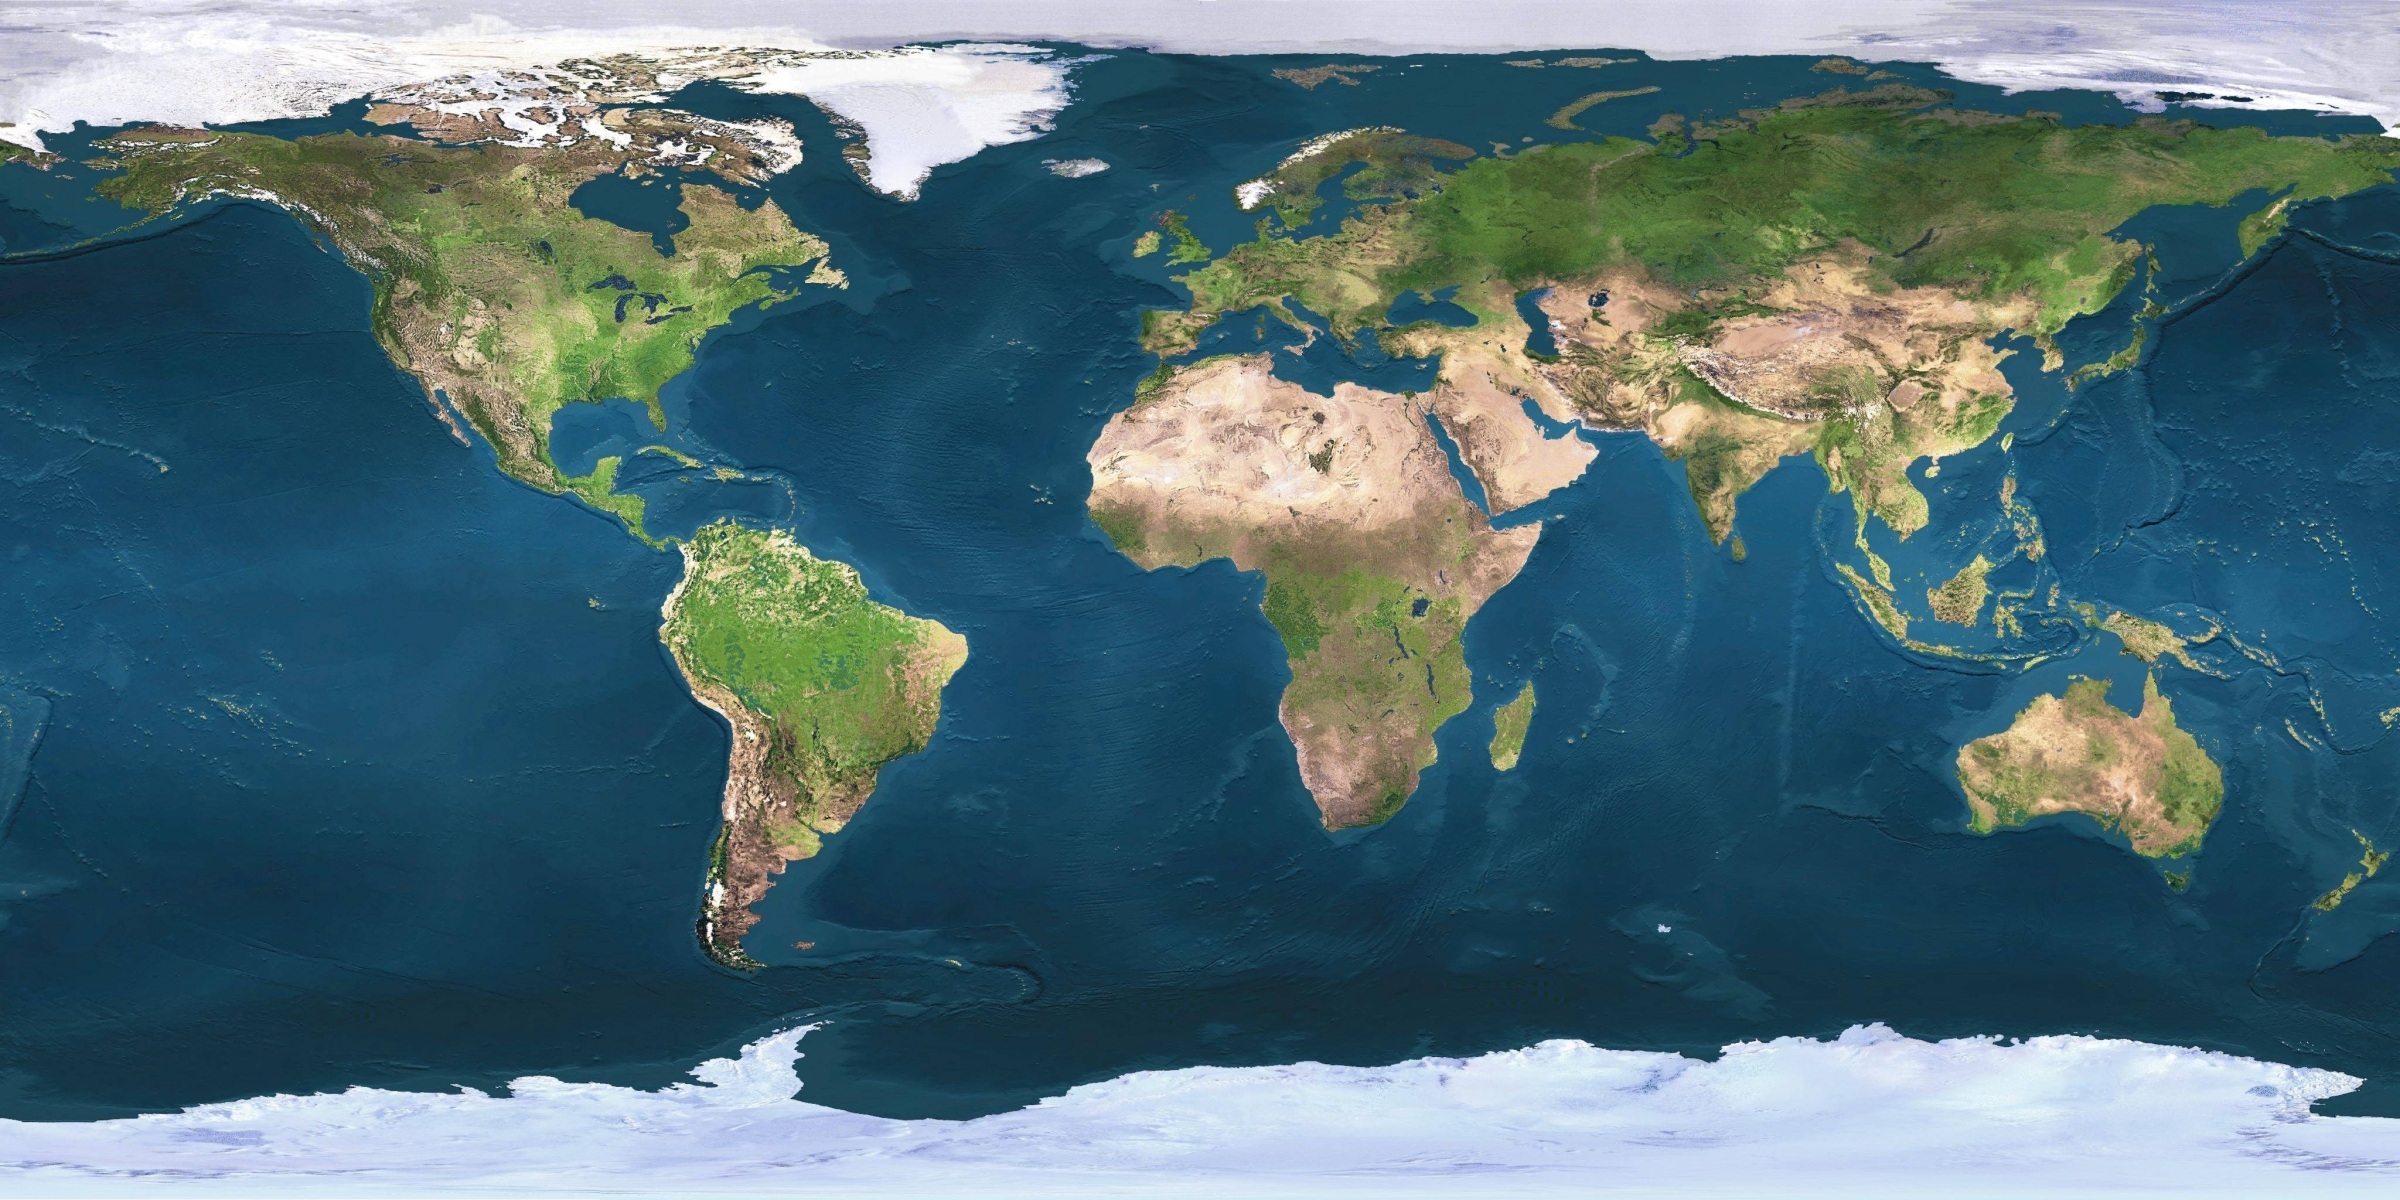
\includegraphics[width = 1.00\textwidth]{p3-img1}
 		\captionof{figure}{\label{fig:IPN}Visualizando la colección (I).} 
	\end{center} 
\end{figure}

 \begin{figure}[H]
	\begin{center}
 		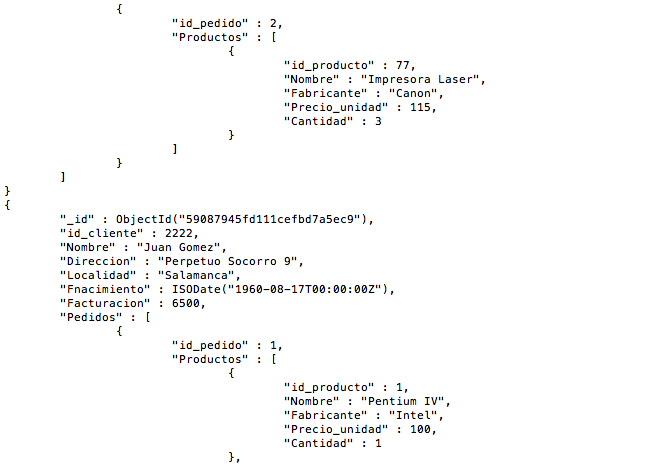
\includegraphics[width = 1.00\textwidth]{p3-img2}
 		\captionof{figure}{\label{fig:IPN}Visualizando la colección (II).} 
	\end{center} 
\end{figure}

 \begin{figure}[H]
	\begin{center}
 		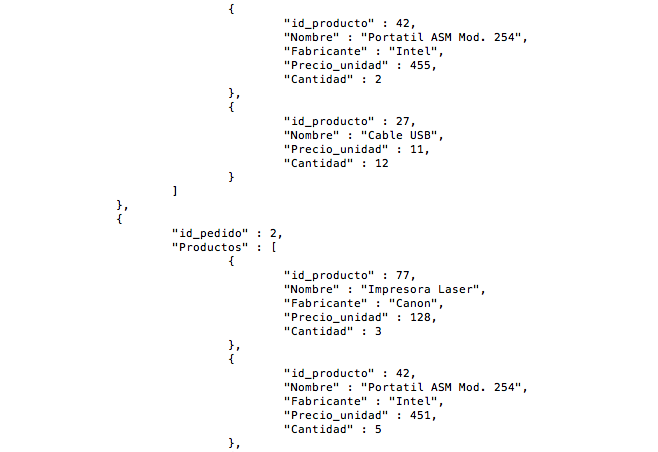
\includegraphics[width = 1.00\textwidth]{p3-img3}
 		\captionof{figure}{\label{fig:IPN}Visualizando la colección (III).} 
	\end{center} 
\end{figure}

 \begin{figure}[H]
	\begin{center}
 		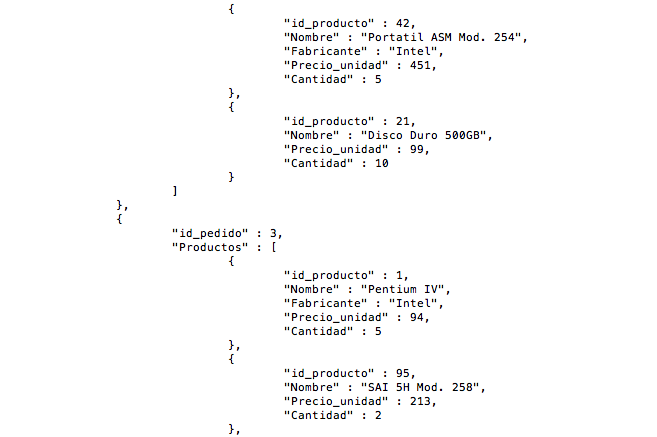
\includegraphics[width = 1.00\textwidth]{p3-img4}
 		\captionof{figure}{\label{fig:IPN}Visualizando la colección (IV).} 
	\end{center} 
\end{figure}

 \begin{figure}[H]
	\begin{center}
 		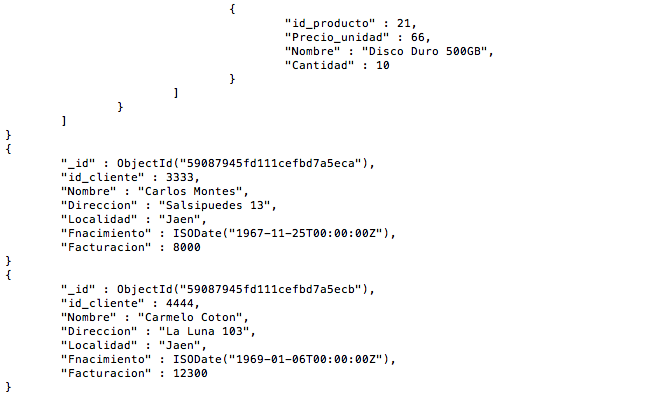
\includegraphics[width = 1.00\textwidth]{p3-img5}
 		\captionof{figure}{\label{fig:IPN}Visualizando la colección (V).} 
	\end{center} 
\end{figure}

 \begin{figure}[H]
	\begin{center}
 		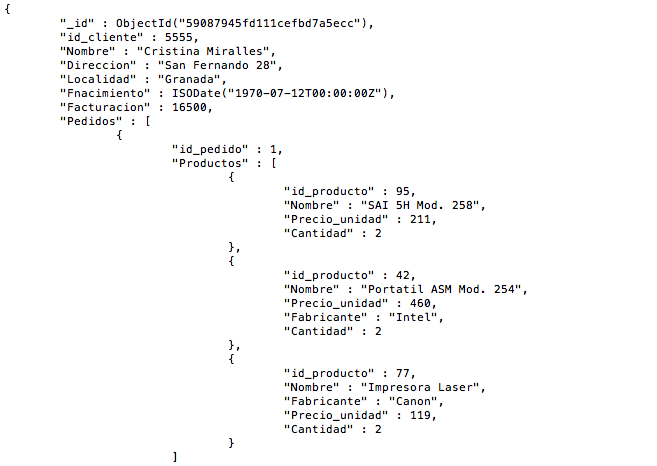
\includegraphics[width = 1.00\textwidth]{p3-img6}
 		\captionof{figure}{\label{fig:IPN}Visualizando la colección (VI).} 
	\end{center} 
\end{figure}

 \begin{figure}[H]
	\begin{center}
 		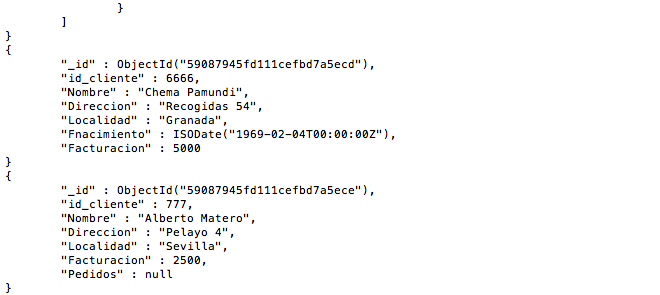
\includegraphics[width = 1.00\textwidth]{p3-img7}
 		\captionof{figure}{\label{fig:IPN}Visualizando la colección (VII).} 
	\end{center} 
\end{figure}


\vspace{4cm}
\subsection{Visualiza sólo el primer documento de la colección. Utiliza los métodos \textbf{.limit()} y \textbf{.findOne()} .} 

 \begin{figure}[H]
	\begin{center}
 		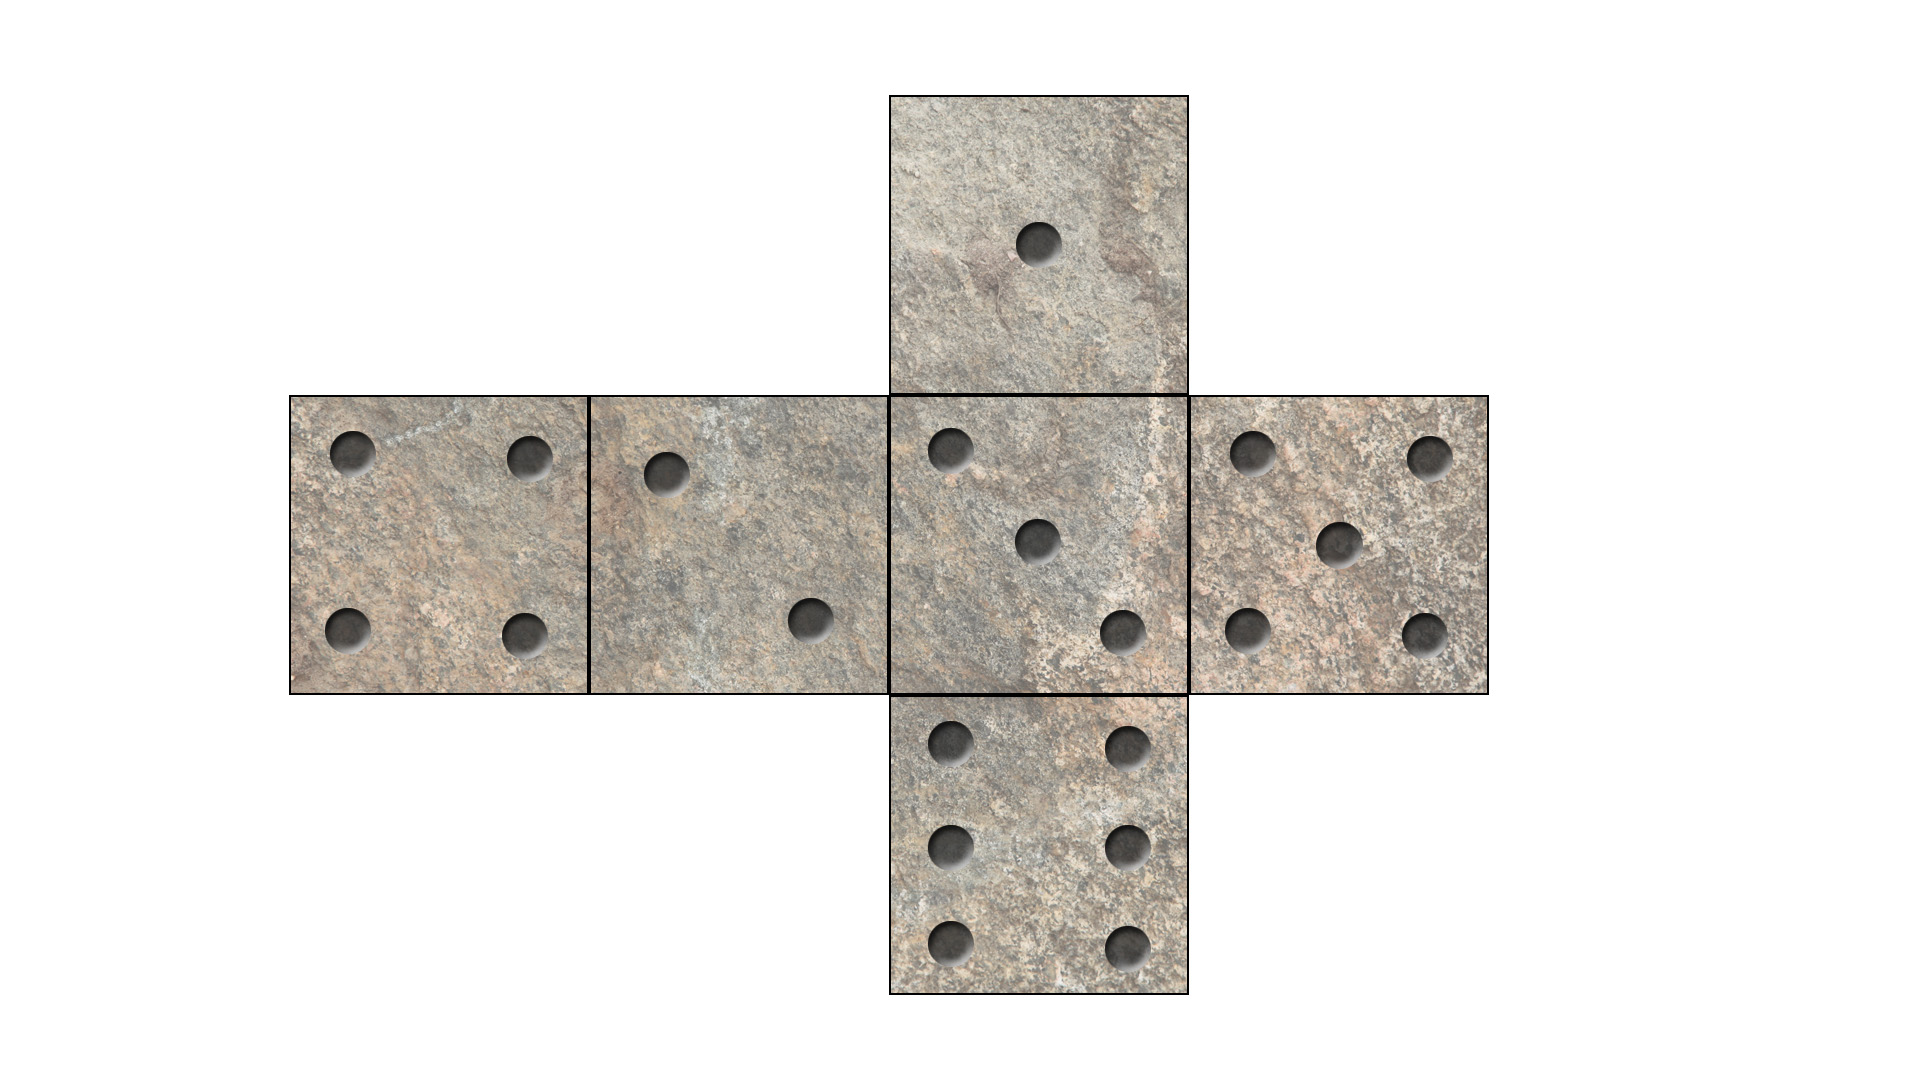
\includegraphics[width = 1.00\textwidth]{p3-img8}
 		\captionof{figure}{\label{fig:IPN}Visualizando el primer documento (I).} 
	\end{center} 
\end{figure}

 \begin{figure}[H]
	\begin{center}
 		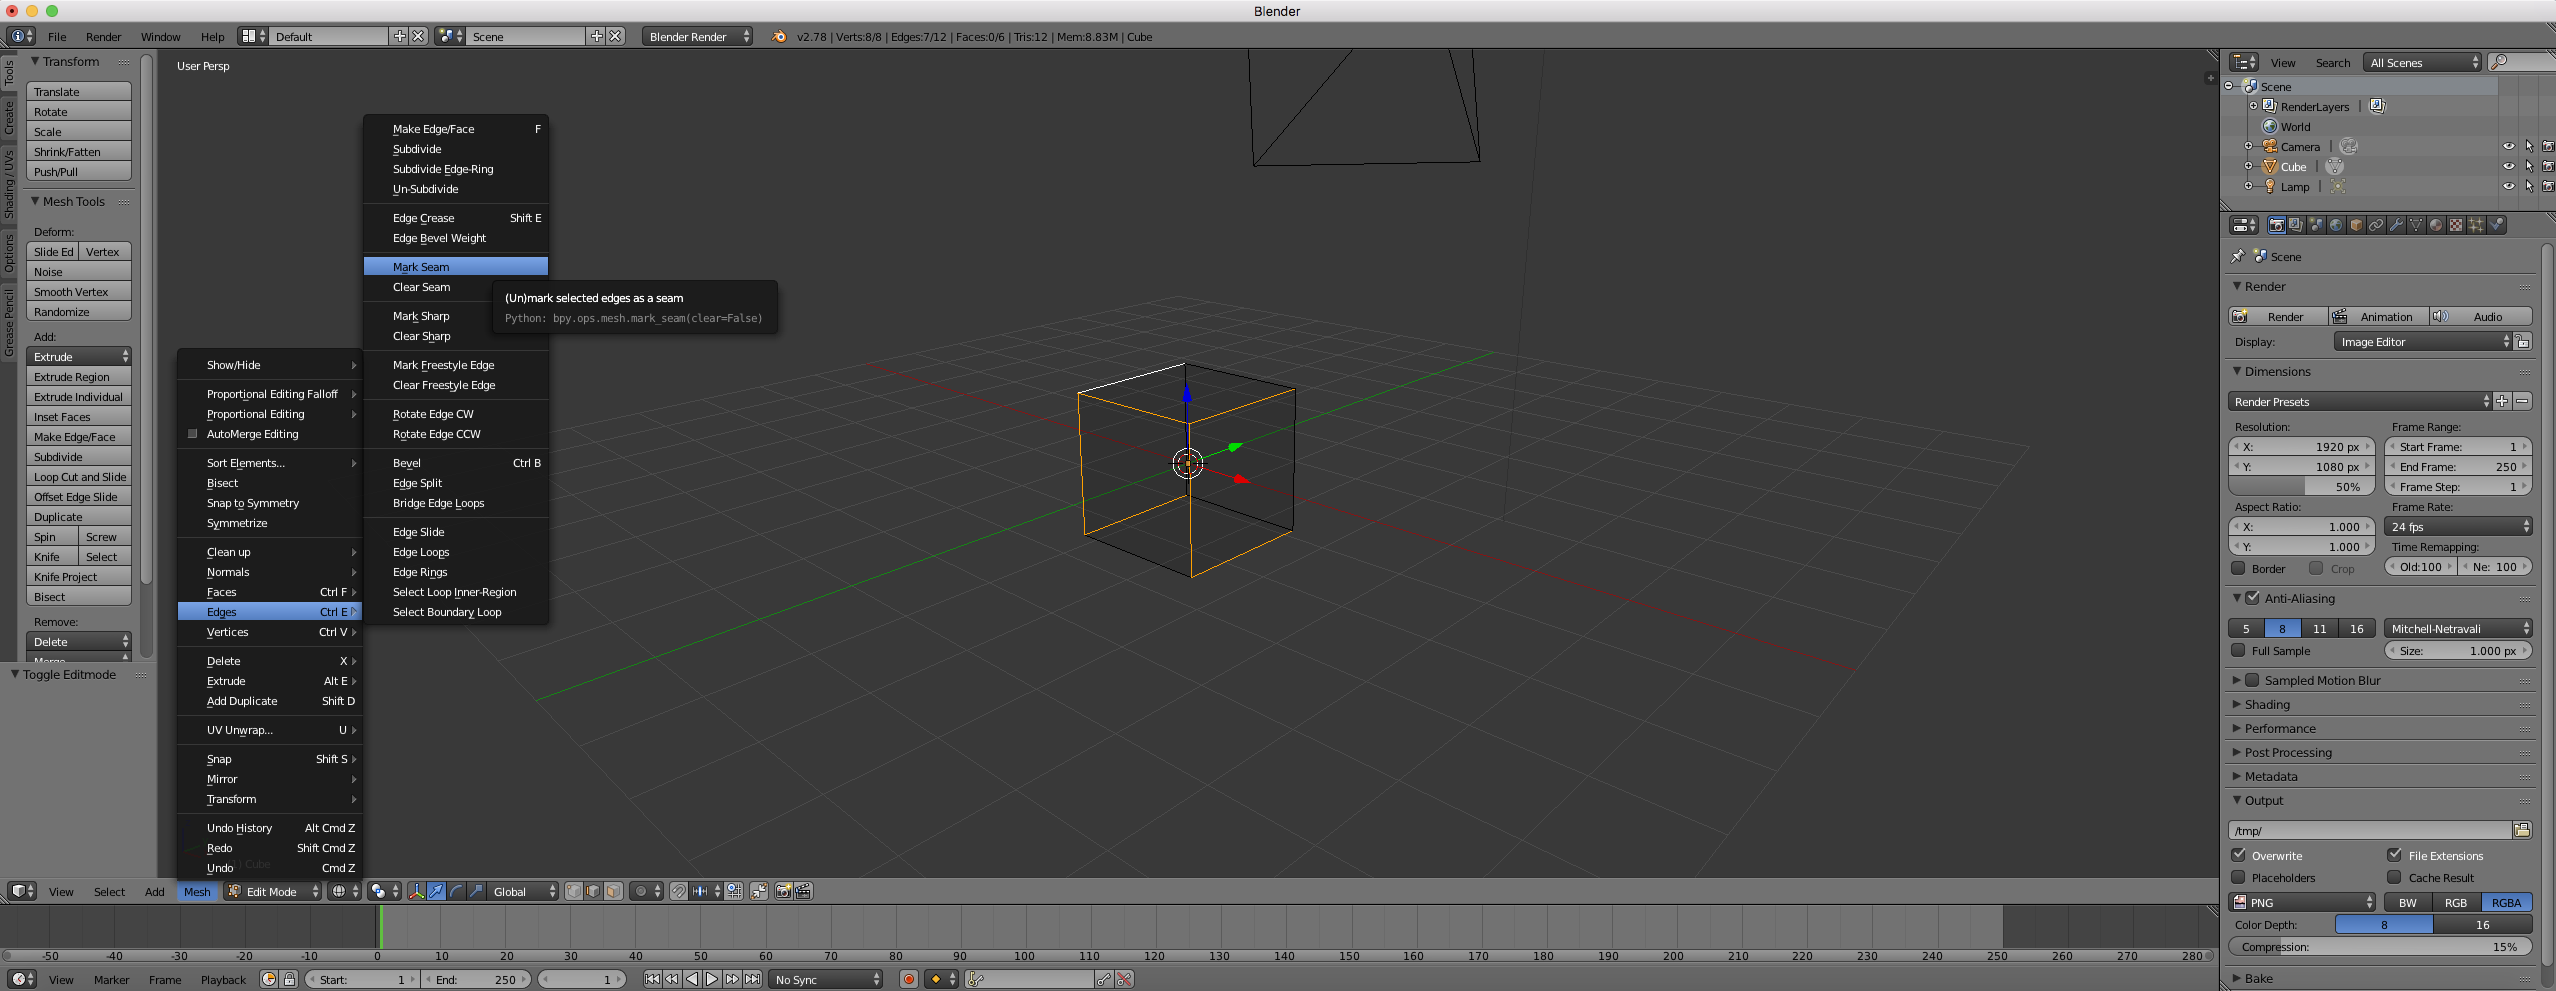
\includegraphics[width = 1.00\textwidth]{p3-img9}
 		\captionof{figure}{\label{fig:IPN}Visualizando el primer documento (II).} 
	\end{center} 
\end{figure}

\vspace{10cm}
\subsection{Visualiza el cliente con el \textbf{id\_cliente = 2222} .}

 \begin{figure}[H]
	\begin{center}
 		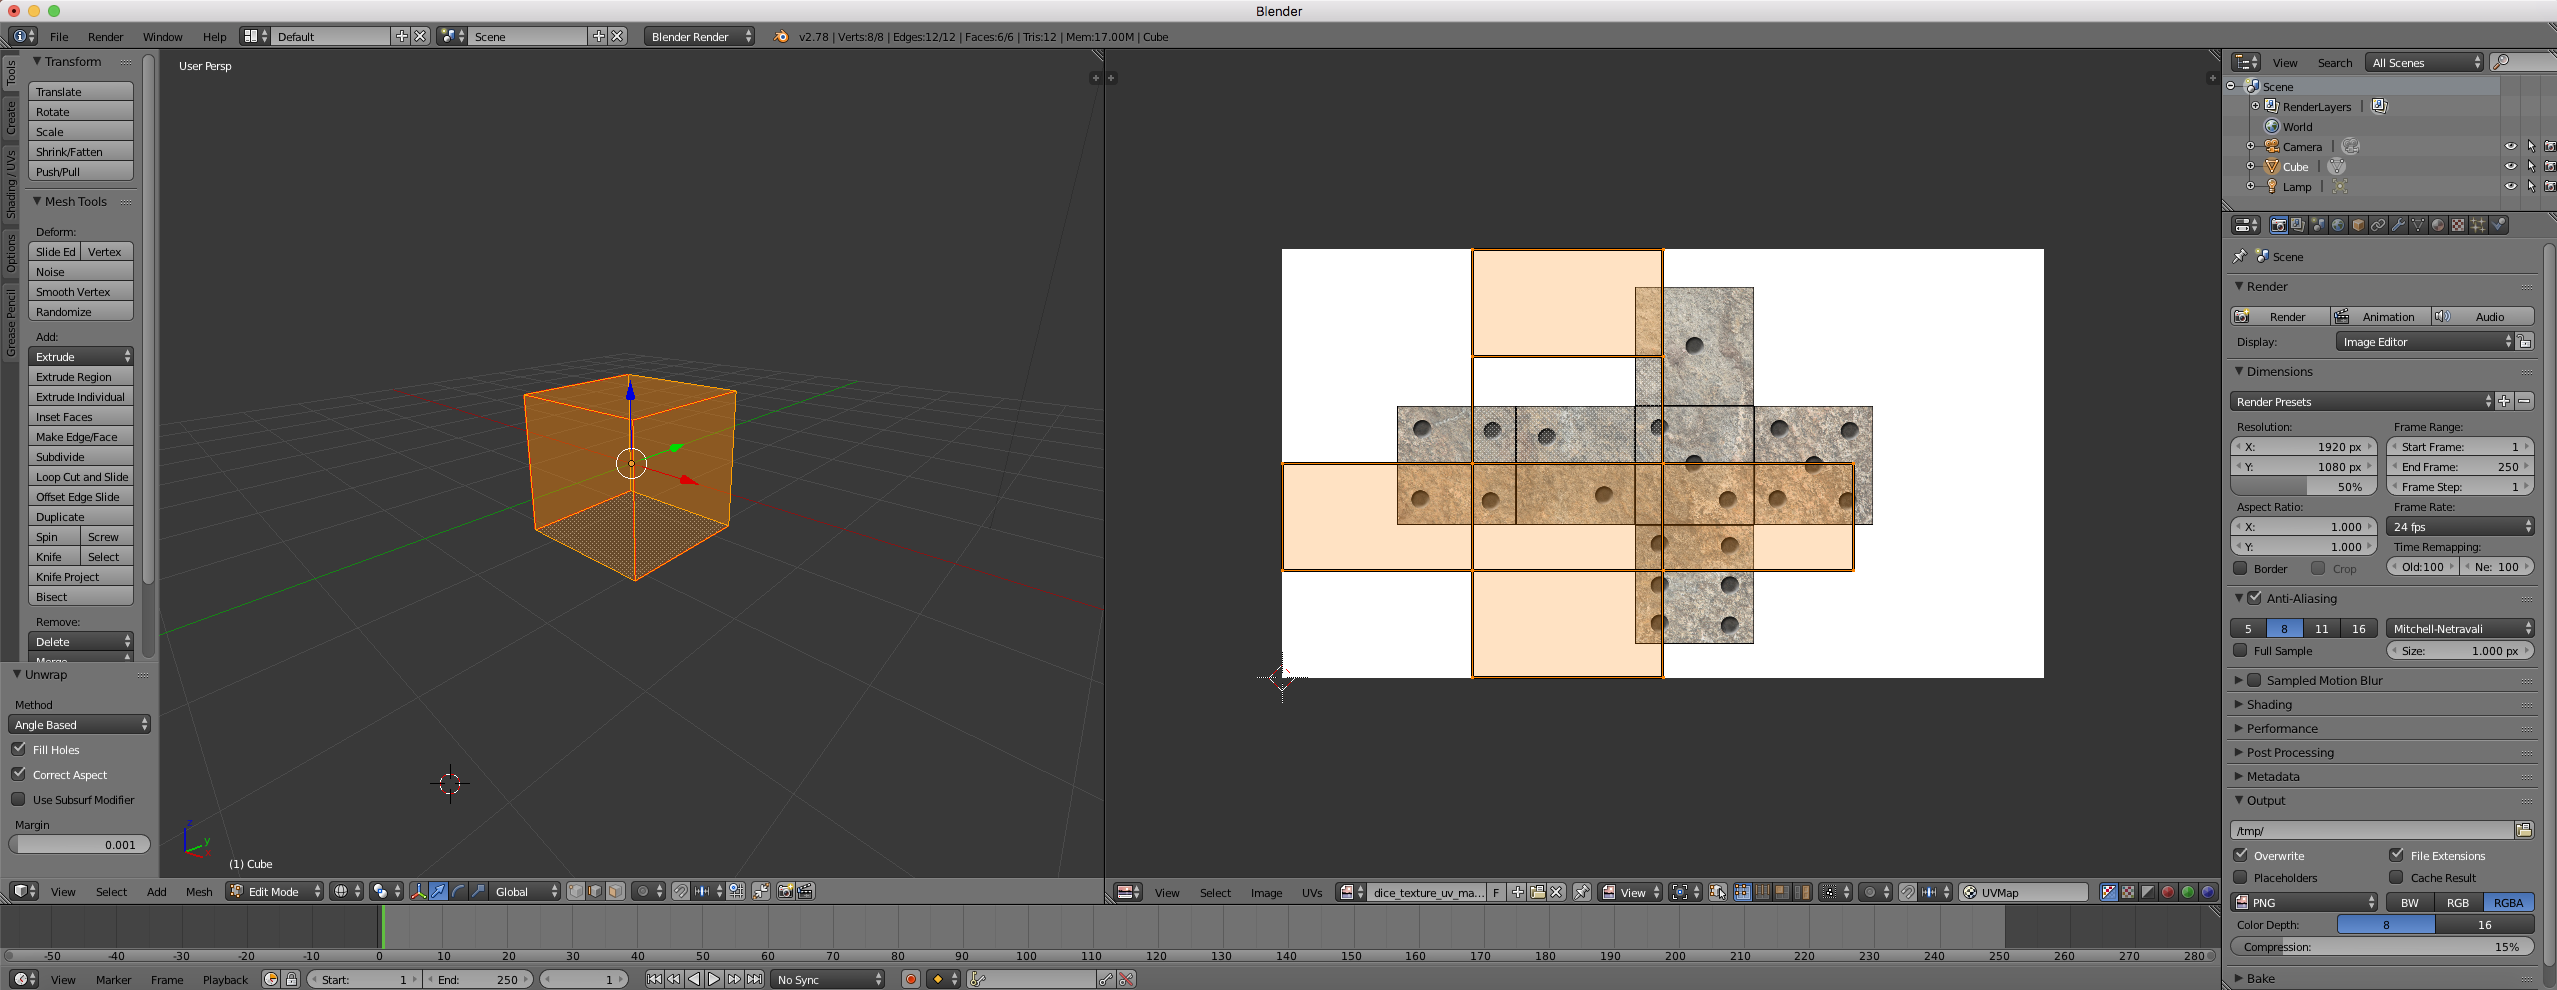
\includegraphics[width = 1.00\textwidth]{p3-img10}
 		\captionof{figure}{\label{fig:IPN}Visualizando los datos del cliente (I).} 
	\end{center} 
\end{figure}

 \begin{figure}[H]
	\begin{center}
 		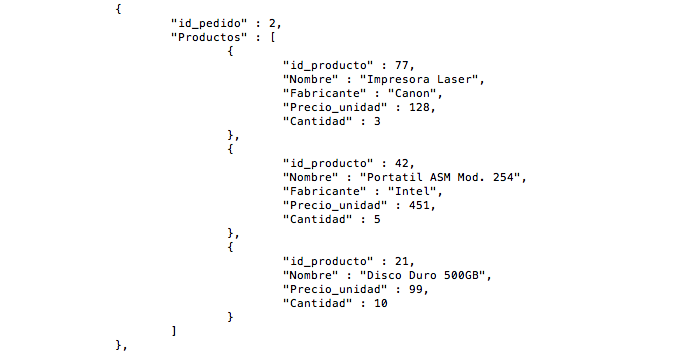
\includegraphics[width = 1.00\textwidth]{p3-img11}
 		\captionof{figure}{\label{fig:IPN}Visualizando los datos del cliente (II).} 
	\end{center} 
\end{figure}

 \begin{figure}[H]
	\begin{center}
 		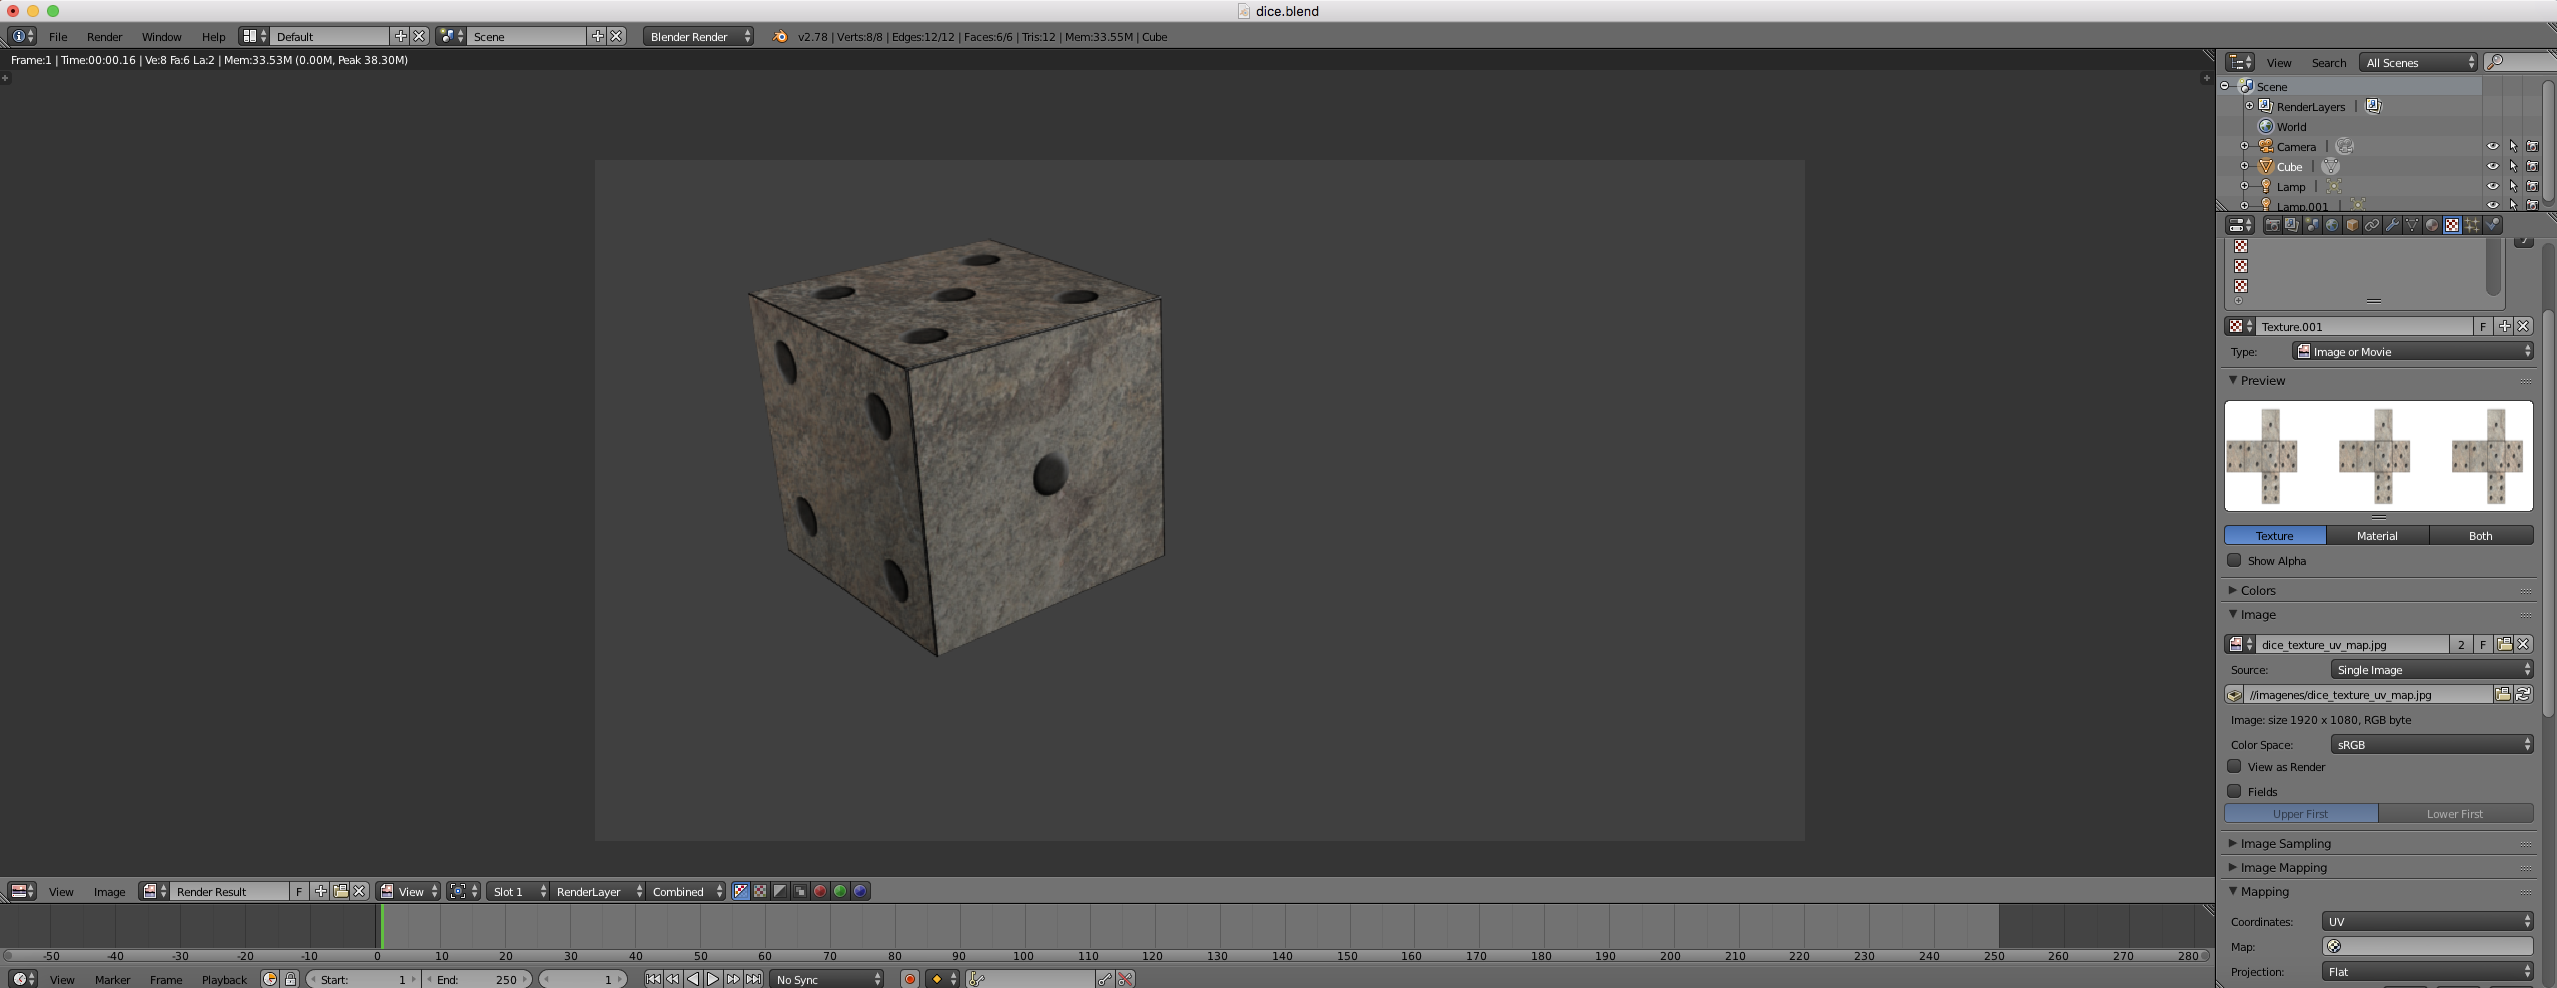
\includegraphics[width = 1.00\textwidth]{p3-img12}
 		\captionof{figure}{\label{fig:IPN}Visualizando los datos del cliente (III).} 
	\end{center} 
\end{figure}

\vspace{4cm}
\subsection{Visualiza los clientes que hayan pedido algún producto de más de 94 euros.}

 \begin{figure}[H]
	\begin{center}
 		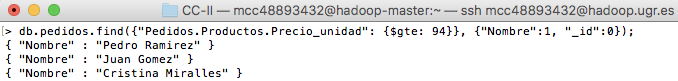
\includegraphics[width = 1.00\textwidth]{p3-img13}
 		\captionof{figure}{\label{fig:IPN}Visualizando los clientes.} 
	\end{center} 
\end{figure}


\subsection{Visualiza los clientes de Jaén o Salamanca (excluye los datos de los pedidos). Utiliza los operadores \$or e \$in .}

 \begin{figure}[H]
	\begin{center}
 		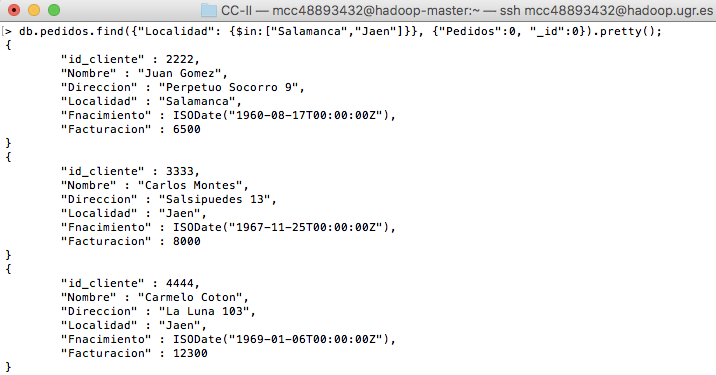
\includegraphics[width = 1.00\textwidth]{p3-img14}
 		\captionof{figure}{\label{fig:IPN}Visualizando los clientes.} 
	\end{center} 
\end{figure}


\subsection{Visualiza los clientes que no tienen campo pedido.}

 \begin{figure}[H]
	\begin{center}
 		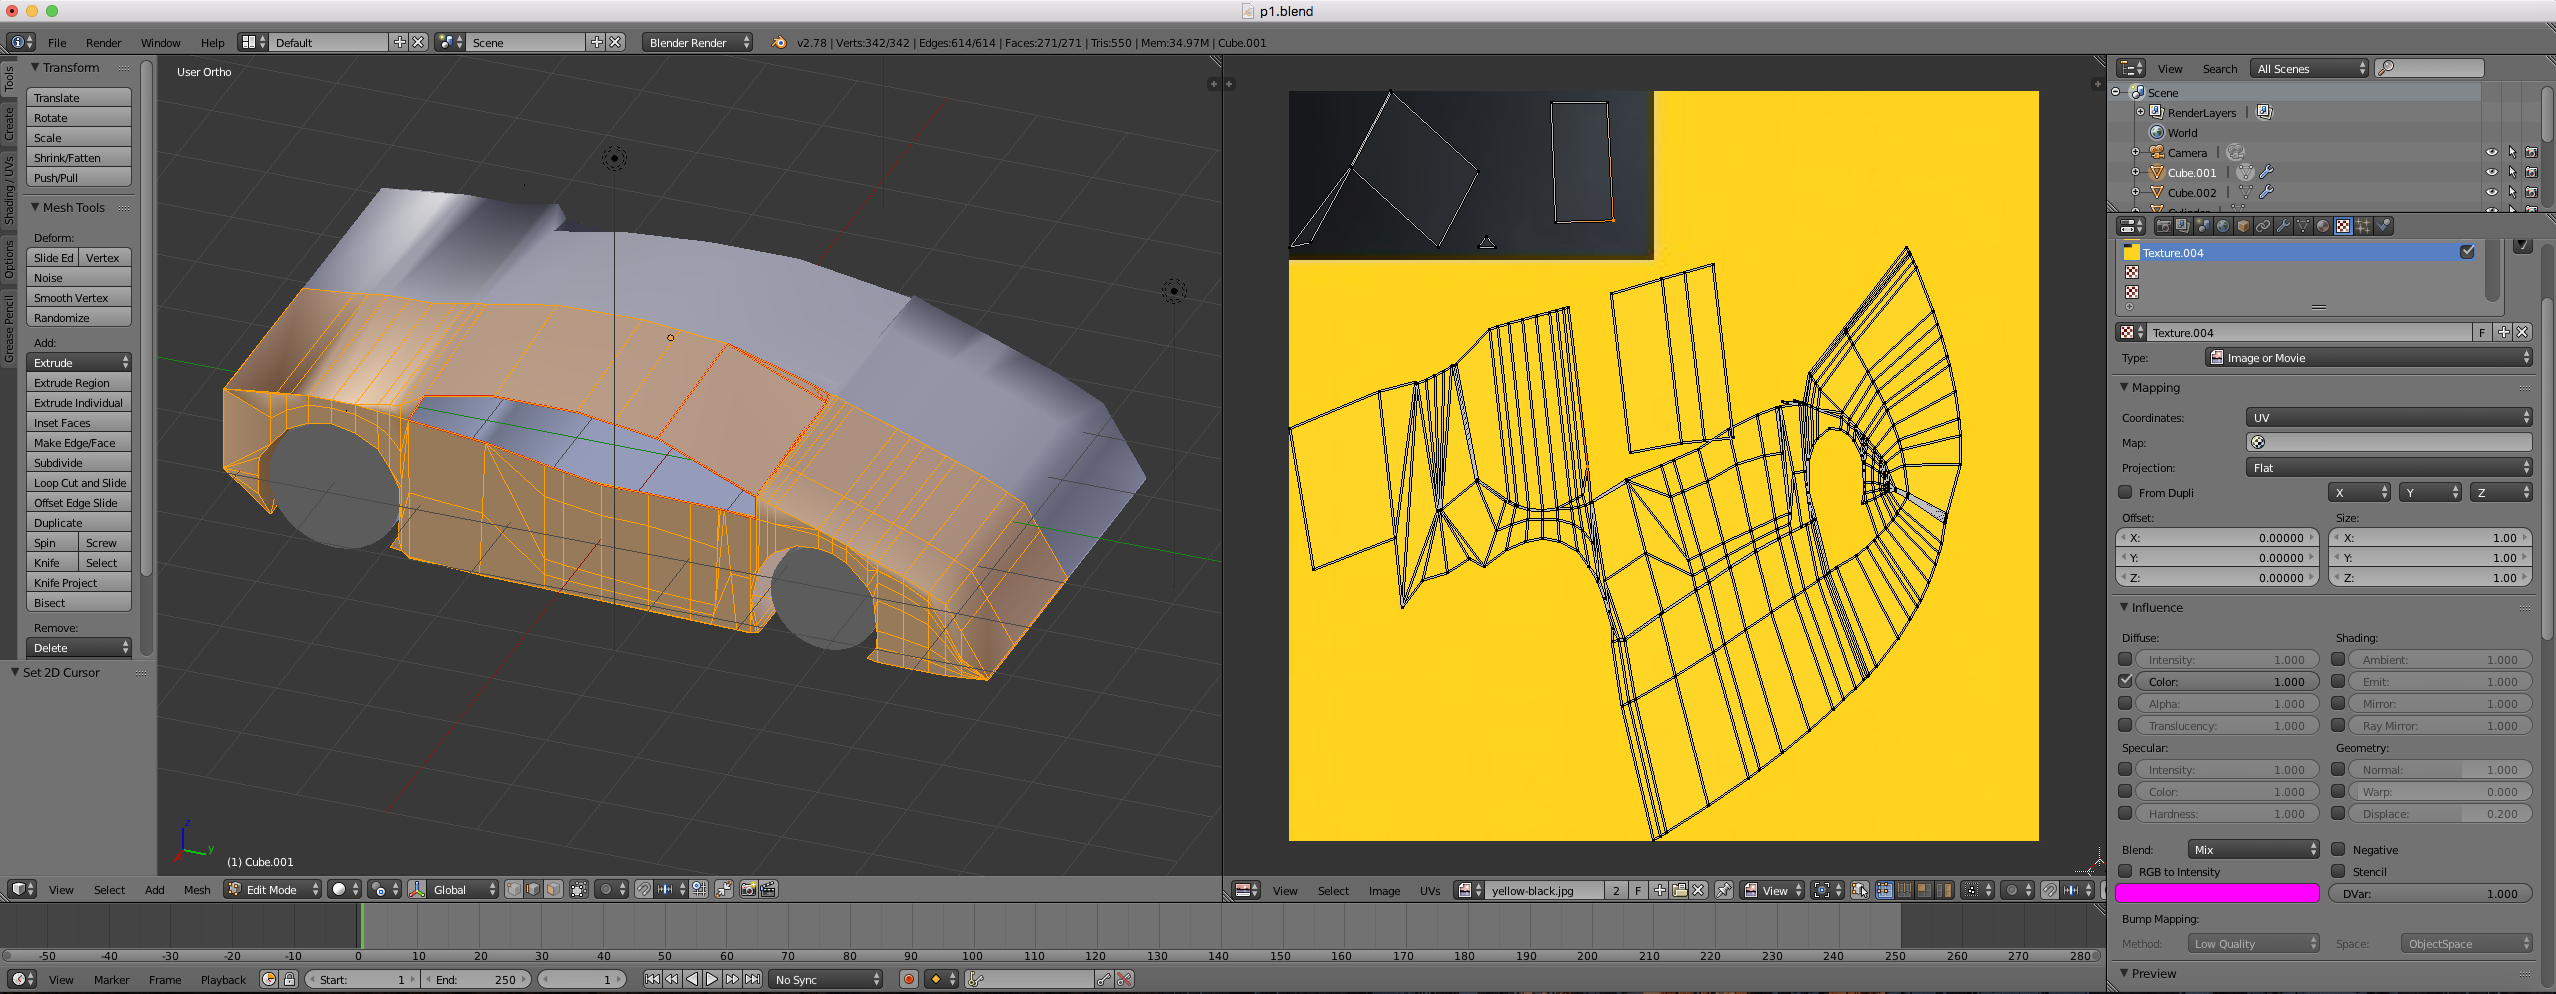
\includegraphics[width = 1.00\textwidth]{p3-img15}
 		\captionof{figure}{\label{fig:IPN}Visualizando los clientes.} 
	\end{center} 
\end{figure}


\subsection{Visualiza los clientes que hayan nacido en 1963.}

 \begin{figure}[H]
	\begin{center}
 		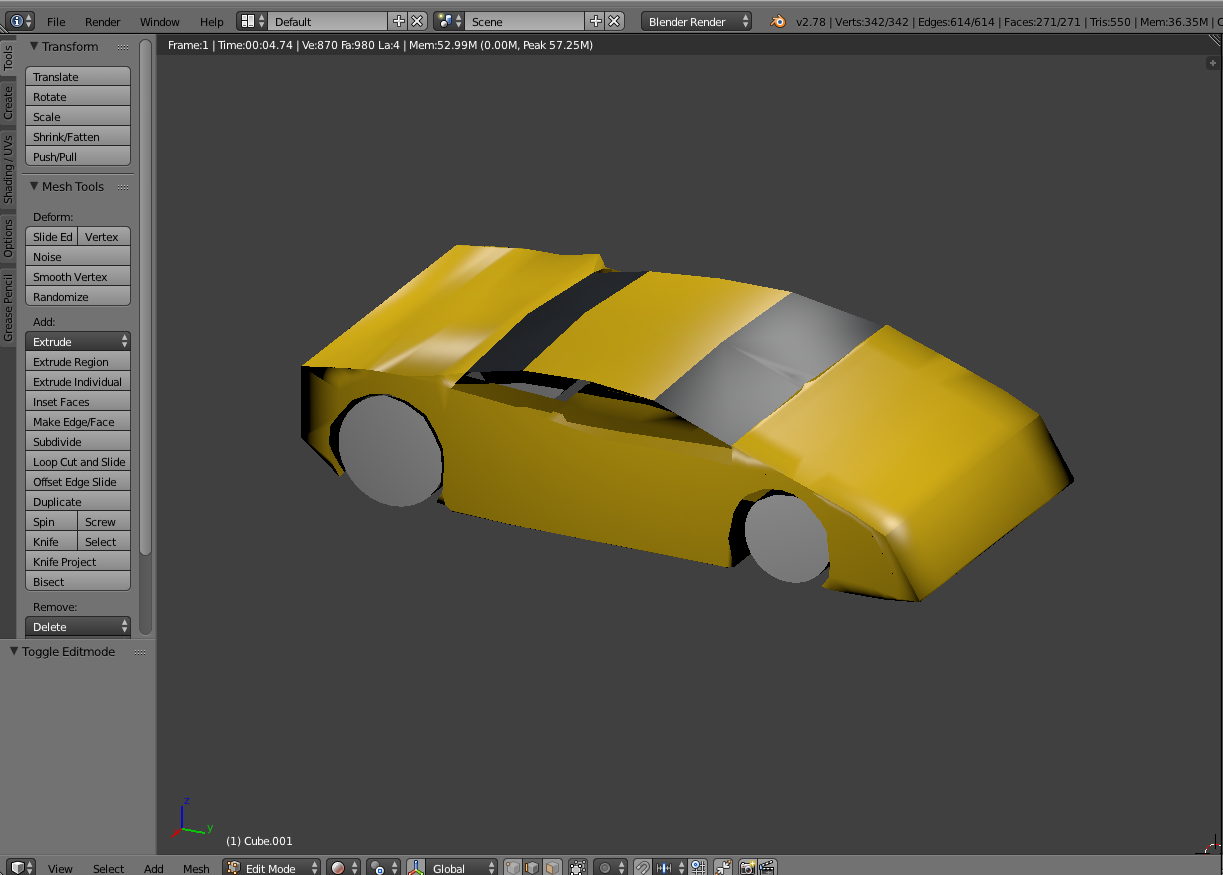
\includegraphics[width = 1.00\textwidth]{p3-img16}
 		\captionof{figure}{\label{fig:IPN}Visualizando los clientes.} 
	\end{center} 
\end{figure}

\subsection{Visualiza los clientes que hayan pedido algún producto fabricado por Canon y algún producto cuyo precio sea inferior a 15 euros.}

 \begin{figure}[H]
	\begin{center}
 		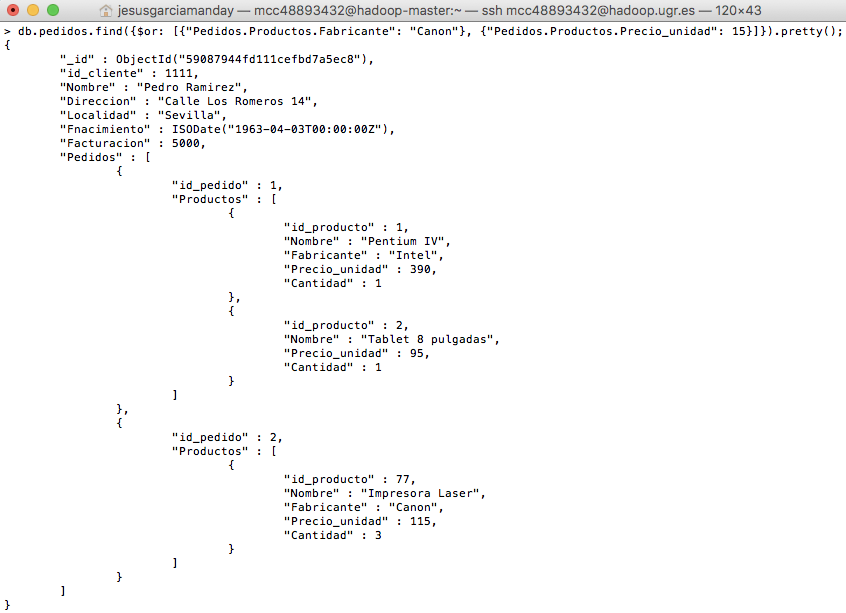
\includegraphics[width = 1.00\textwidth]{p3-img17}
 		\captionof{figure}{\label{fig:IPN}Visualizando los clientes (I).} 
	\end{center} 
\end{figure}

 \begin{figure}[H]
	\begin{center}
 		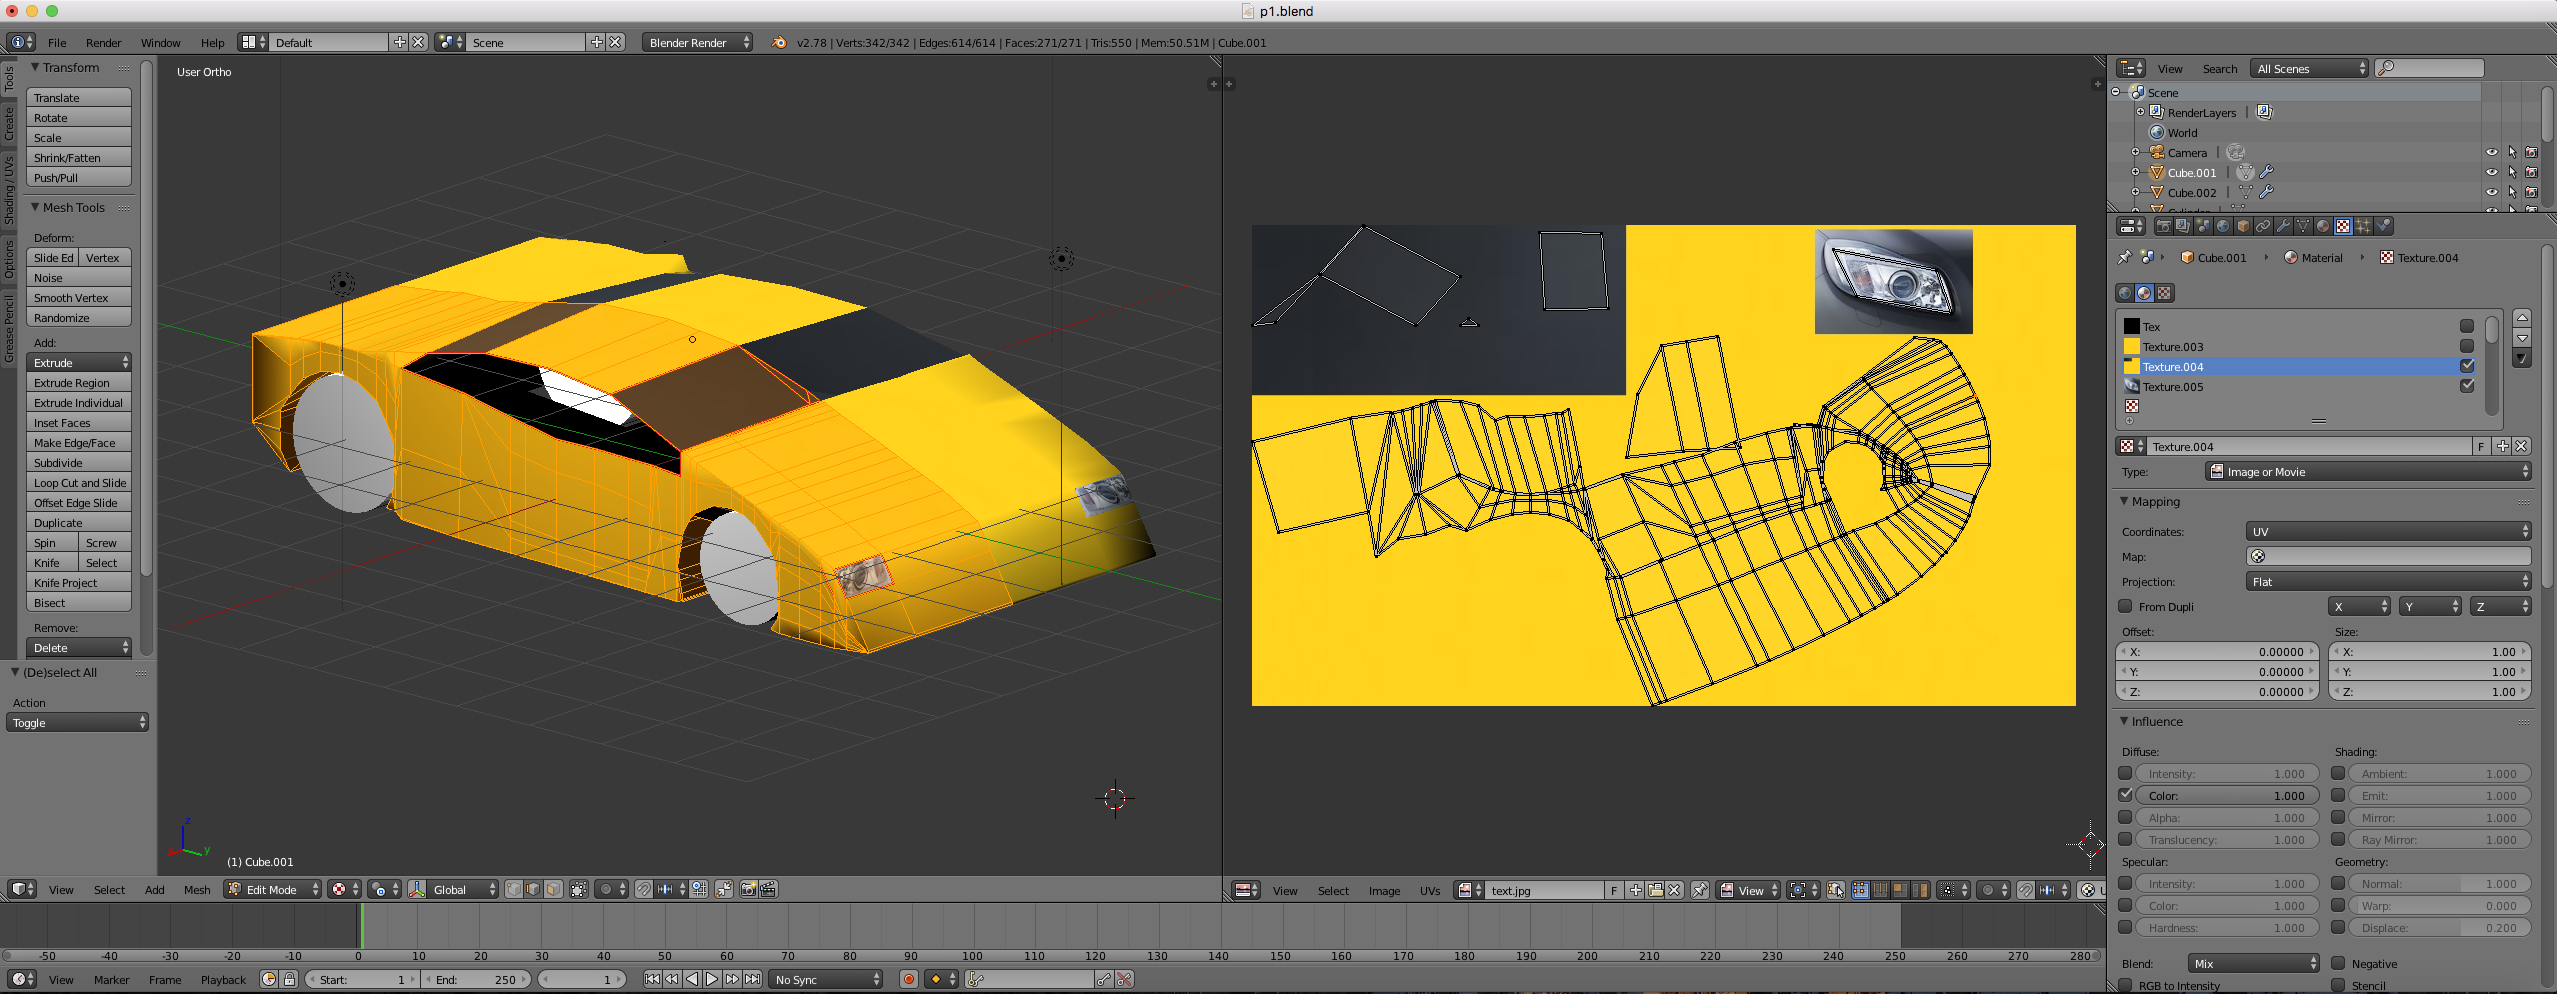
\includegraphics[width = 1.00\textwidth]{p3-img18}
 		\captionof{figure}{\label{fig:IPN}Visualizando los clientes (II).} 
	\end{center} 
\end{figure}

 \begin{figure}[H]
	\begin{center}
 		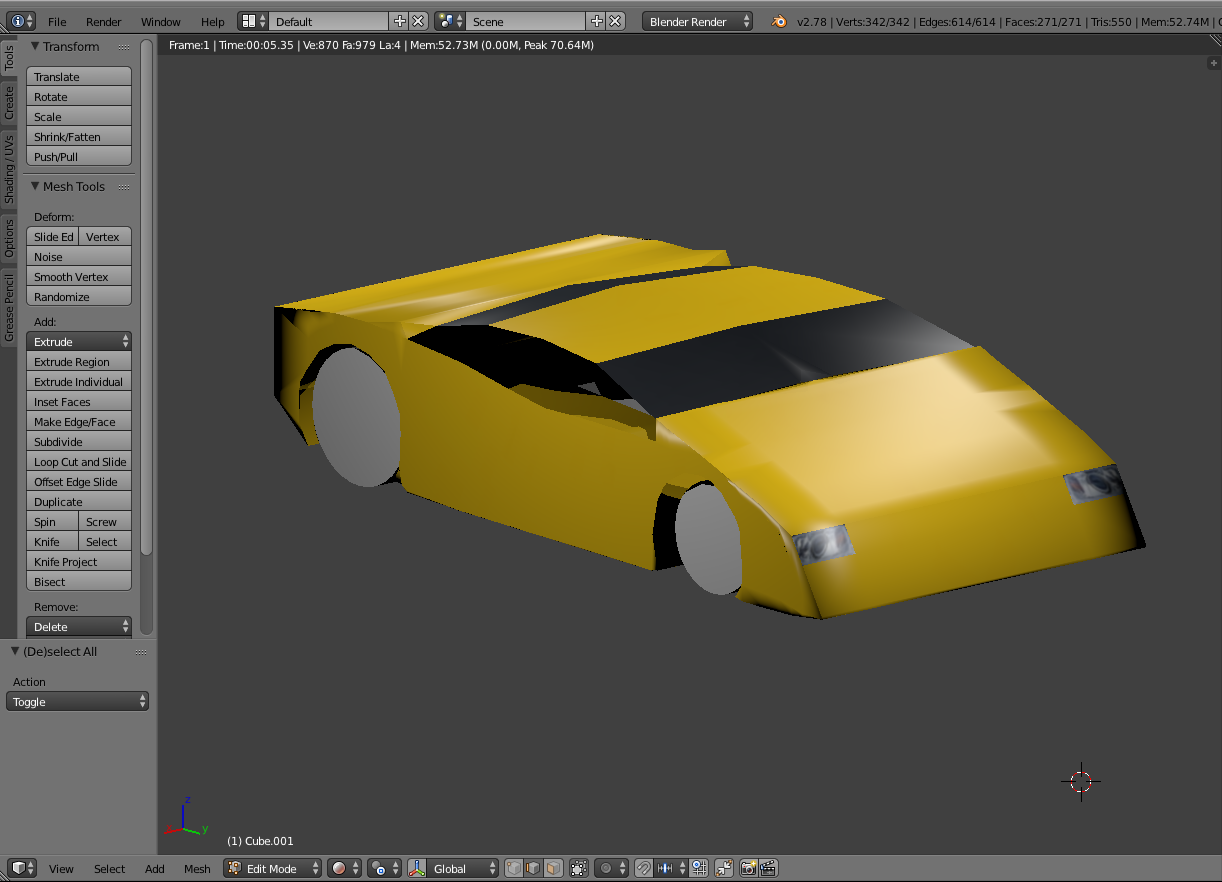
\includegraphics[width = 1.00\textwidth]{p3-img19}
 		\captionof{figure}{\label{fig:IPN}Visualizando los clientes (III).} 
	\end{center} 
\end{figure}

 \begin{figure}[H]
	\begin{center}
 		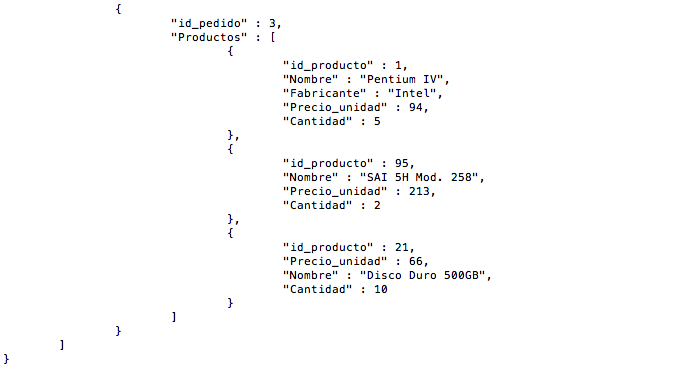
\includegraphics[width = 1.00\textwidth]{p3-img20}
 		\captionof{figure}{\label{fig:IPN}Visualizando los clientes (IV).} 
	\end{center} 
\end{figure}

 \begin{figure}[H]
	\begin{center}
 		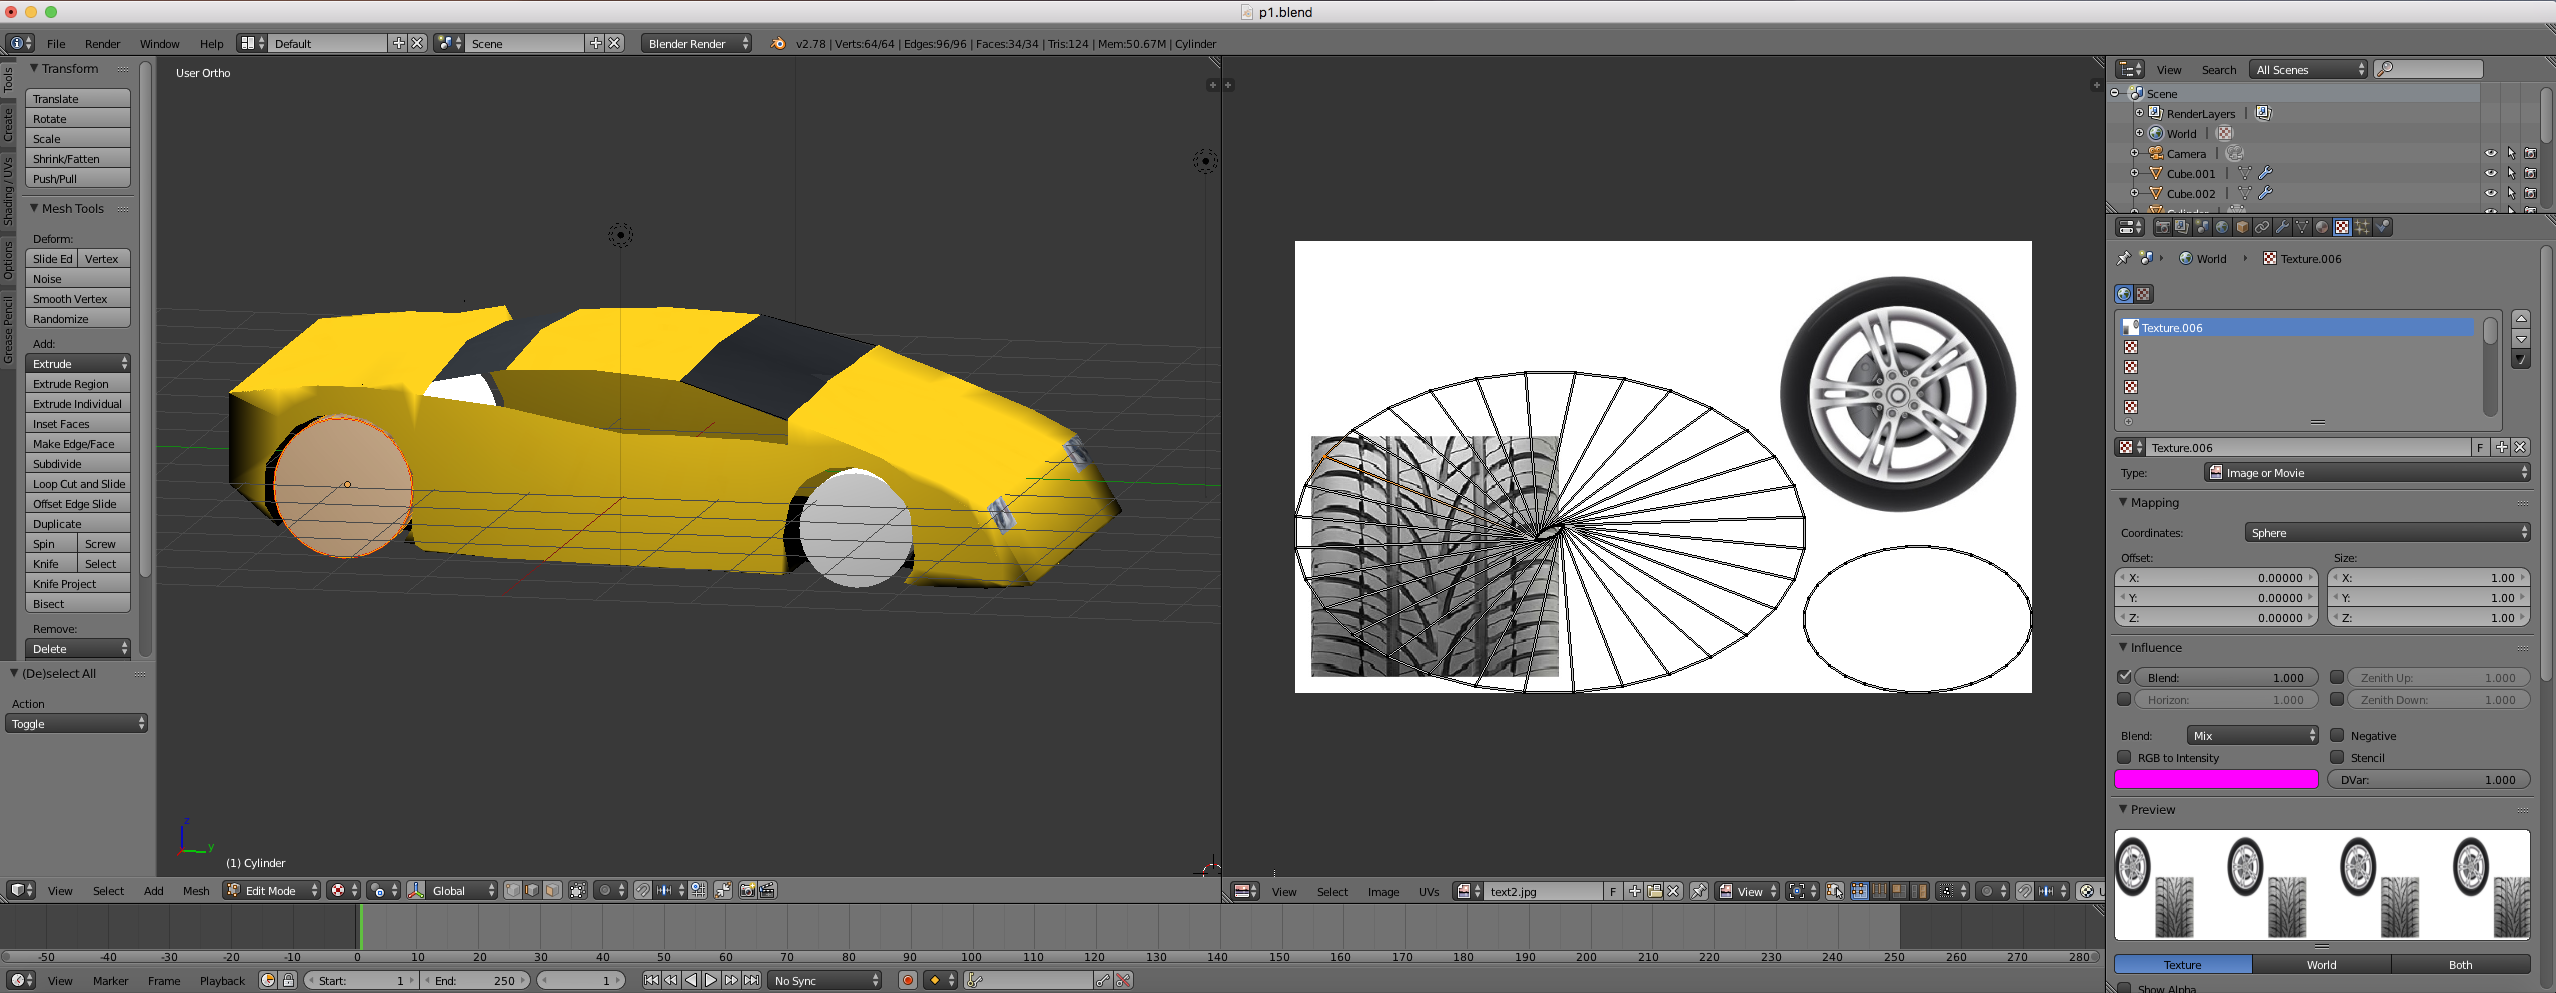
\includegraphics[width = 1.00\textwidth]{p3-img21}
 		\captionof{figure}{\label{fig:IPN}Visualizando los clientes (V).} 
	\end{center} 
\end{figure}


\subsection{Datos personales (id\_cliente, Nombre, Dirección, Localidad y Fnacimiento) de los clientes cuyo nombre empieza por la cadena "c" (No distinguir entre mayúsculas y minúsculas).}

 \begin{figure}[H]
	\begin{center}
 		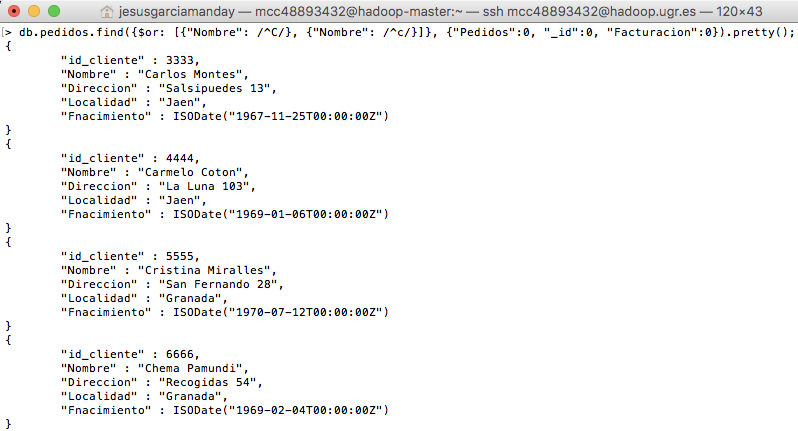
\includegraphics[width = 1.00\textwidth]{p3-img22}
 		\captionof{figure}{\label{fig:IPN}Visualizando los clientes.} 
	\end{center} 
\end{figure}


\subsection{Visualiza los datos personales de los clientes (excluyendo \_id). Limita los documentos a 4.}

 \begin{figure}[H]
	\begin{center}
 		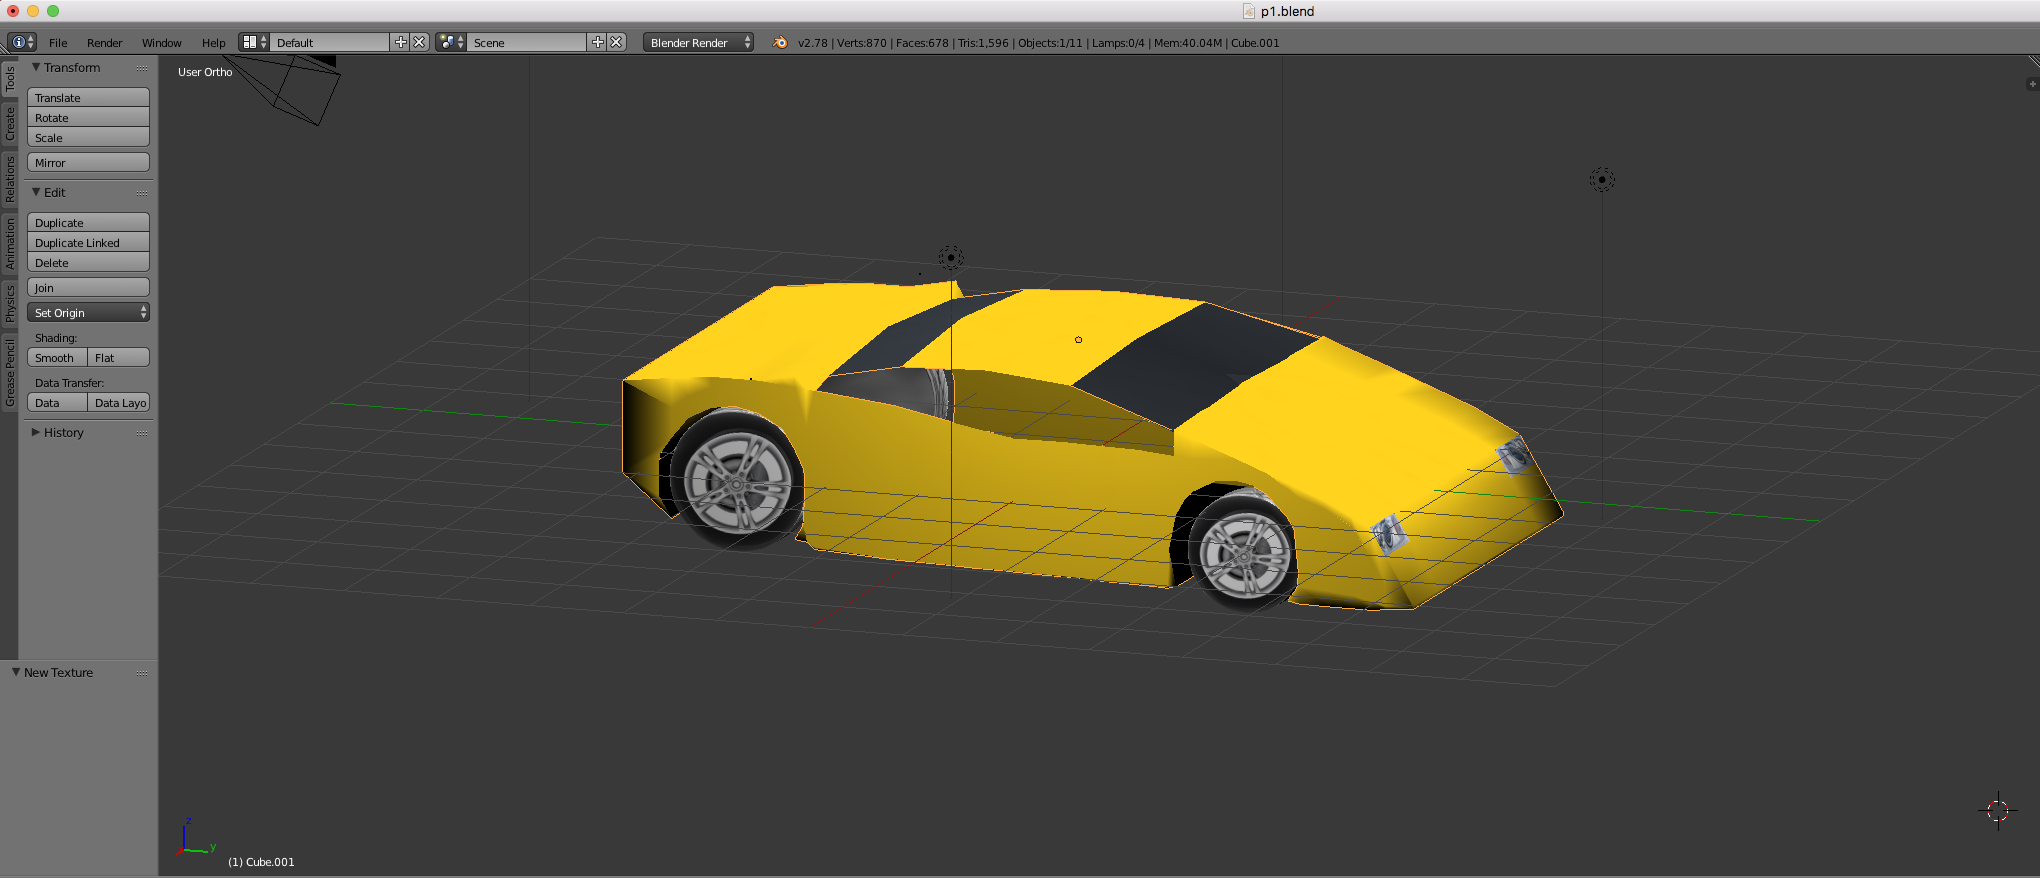
\includegraphics[width = 1.00\textwidth]{p3-img23}
 		\captionof{figure}{\label{fig:IPN}Visualizando los datos personales de los clientes.} 
	\end{center} 
\end{figure}

\subsection{Ídem anterior pero ordenando los documentos por Localidad (ascendente) e \textbf{id\_cliente} (descendente).}

 \begin{figure}[H]
	\begin{center}
 		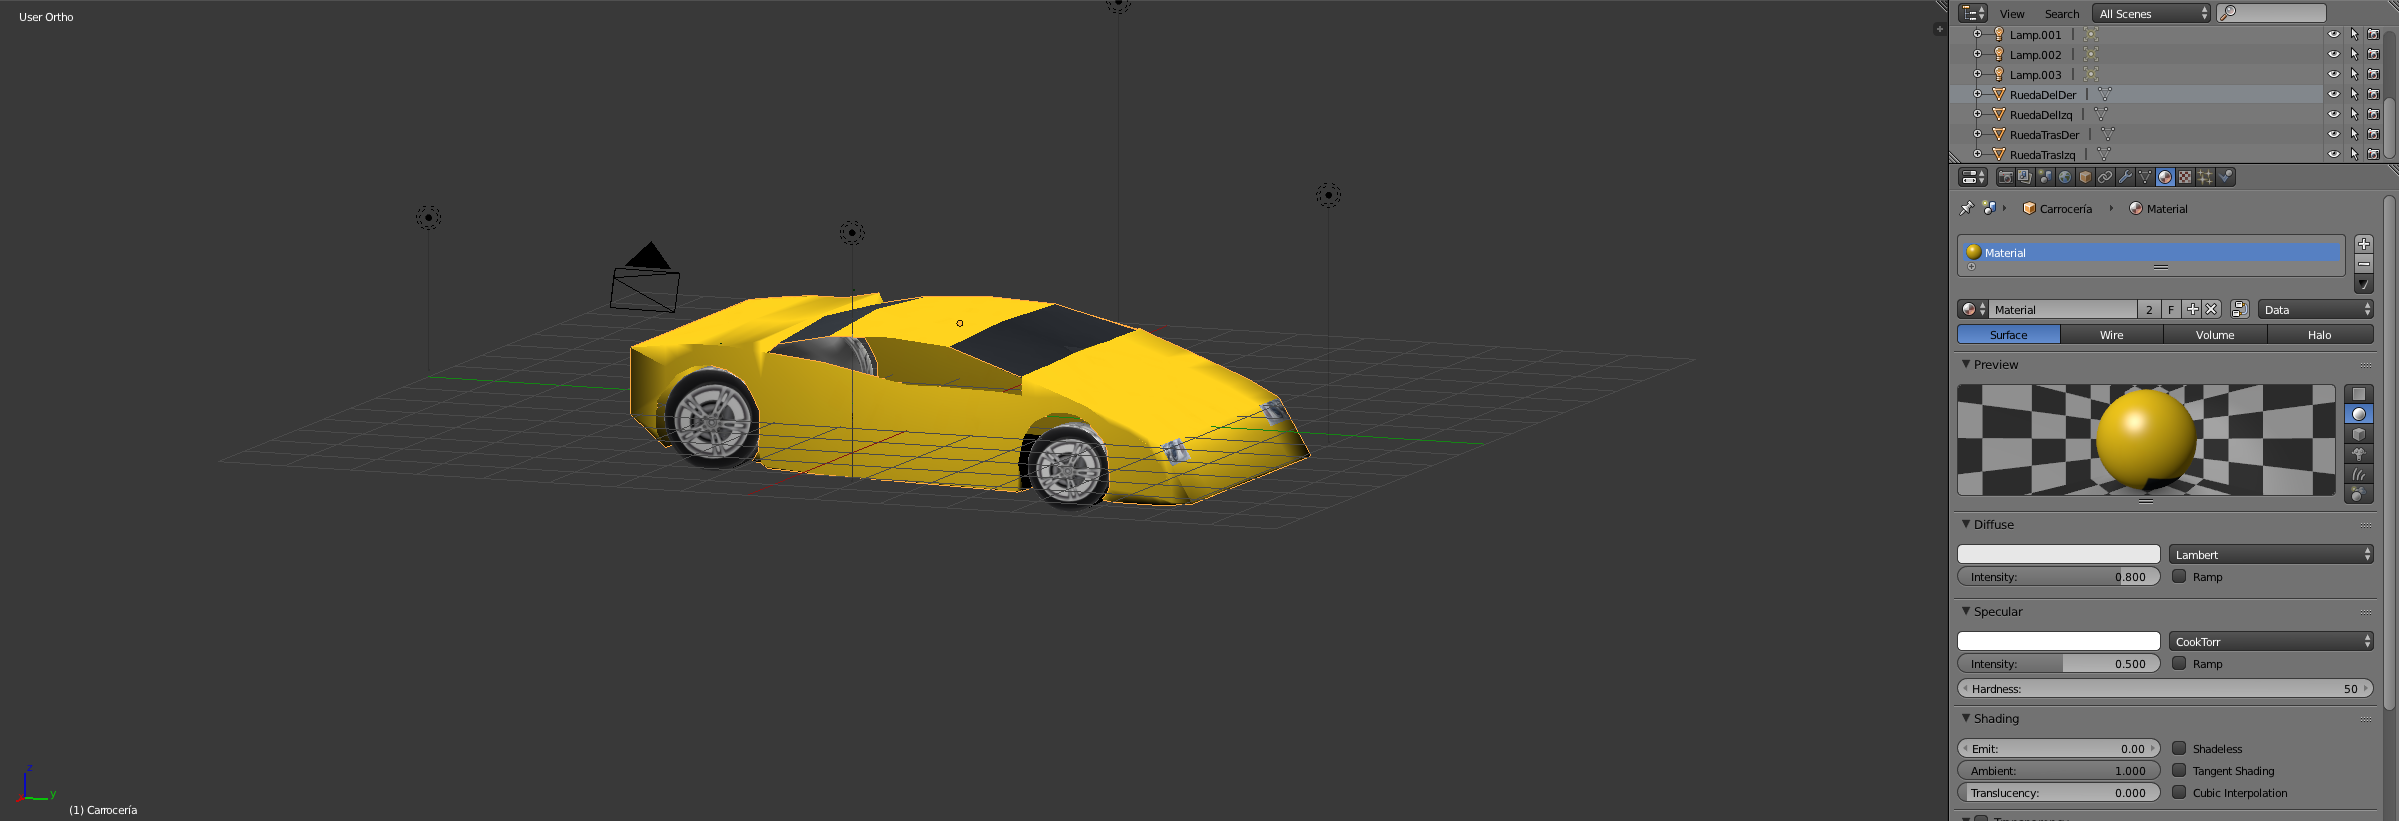
\includegraphics[width = 1.00\textwidth]{p3-img24}
 		\captionof{figure}{\label{fig:IPN}Visualizando los datos personales de los clientes ascendentemente por \textbf{Localidad}.} 
	\end{center} 
\end{figure}

\begin{figure}[H]
	\begin{center}
 		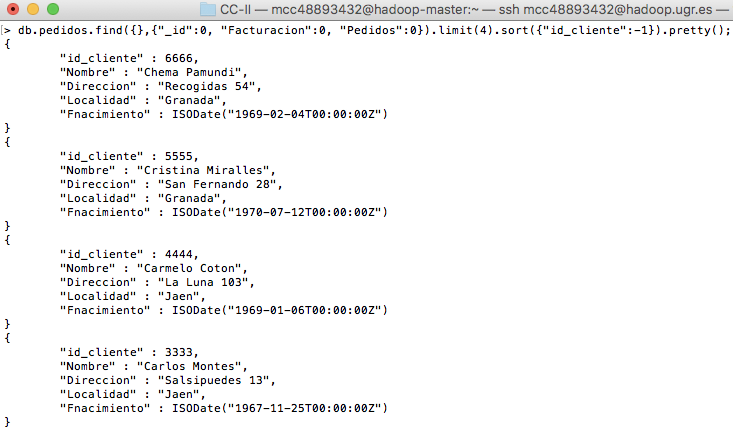
\includegraphics[width = 1.00\textwidth]{p3-img25}
 		\captionof{figure}{\label{fig:IPN}Visualizando los datos personales de los descendentemente por \textbf{id\_cliente}.} 
	\end{center} 
\end{figure}



\section{Agregación.} 

A partir de la colección \textbf{pedidos} utilizaremos consultas más complejas por medio de los operadores de agregación (pipeline). 

\subsection{Nº total de clientes.}

\begin{figure}[H]
	\begin{center}
 		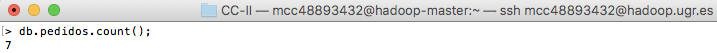
\includegraphics[width = 1.00\textwidth]{p3-img26}
 		\captionof{figure}{\label{fig:IPN}Visualizando el numero de clientes.} 
	\end{center} 
\end{figure}


\subsection{Nº total de clientes de Jaén}

\begin{figure}[H]
	\begin{center}
 		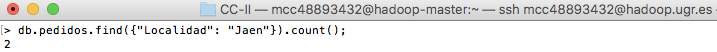
\includegraphics[width = 1.00\textwidth]{p3-img27}
 		\captionof{figure}{\label{fig:IPN}Visualizando el numero de clientes.} 
	\end{center} 
\end{figure}


\subsection{Facturación total clientes por localidad.}

\begin{figure}[H]
	\begin{center}
 		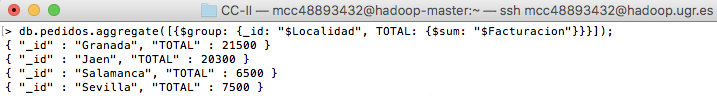
\includegraphics[width = 1.00\textwidth]{p3-img28}
 		\captionof{figure}{\label{fig:IPN}Visualizando las localidades y el total de facturación.} 
	\end{center} 
\end{figure}


\subsection{Facturación media de clientes por localidad para las localidades distintas a Jaén con facturación media mayor de 5000. Ordenación por Localidad descendente. Eliminar el \_id y poner el nombre en mayúsculas.}

\begin{figure}[H]
	\begin{center}
 		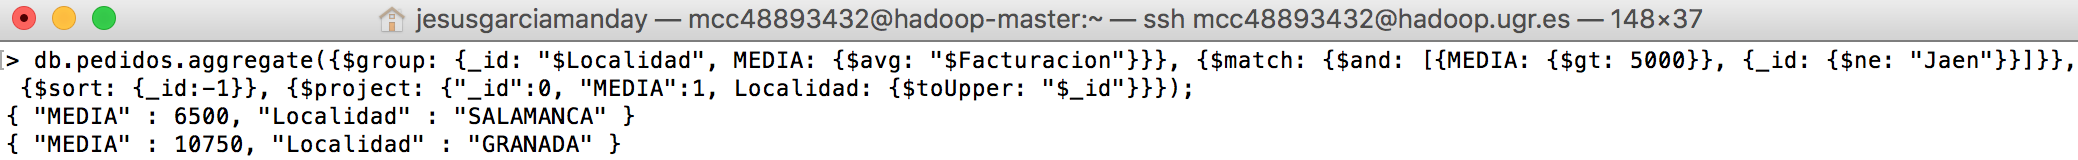
\includegraphics[width = 1.00\textwidth]{p3-img29}
 		\captionof{figure}{\label{fig:IPN}Visualizando las localidades y facturación media.} 
	\end{center} 
\end{figure}


\subsection{Calcula la cantidad total facturada por cada cliente (uso de ''unwind'').}

\begin{figure}[H]
	\begin{center}
 		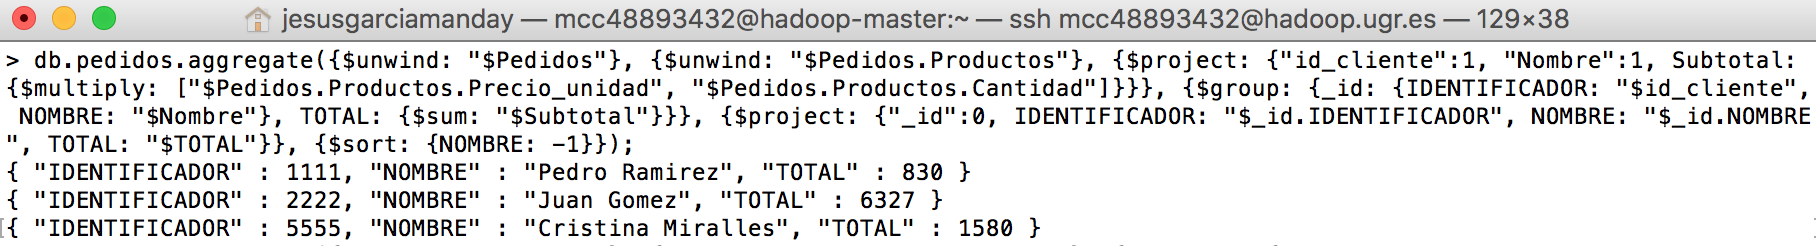
\includegraphics[width = 1.00\textwidth]{p3-img30}
 		\captionof{figure}{\label{fig:IPN}Visualizando los clientes y el total.} 
	\end{center} 
\end{figure}

\section{MapReduce.}

Vamos a utilizar la base de datos libre \textbf{GeoWorldMap} de \textbf{GeoBytes}. Es una base de datos de países, con sus estados/regiones y ciudades importantes. 

\subsection{Encontrar las ciudades más cercanas sobre la colección recién creada mediante un enfoque MapReduce conforme a los pasos que se ilustran en el tutoriak práctico.}

\begin{figure}[H]
	\begin{center}
 		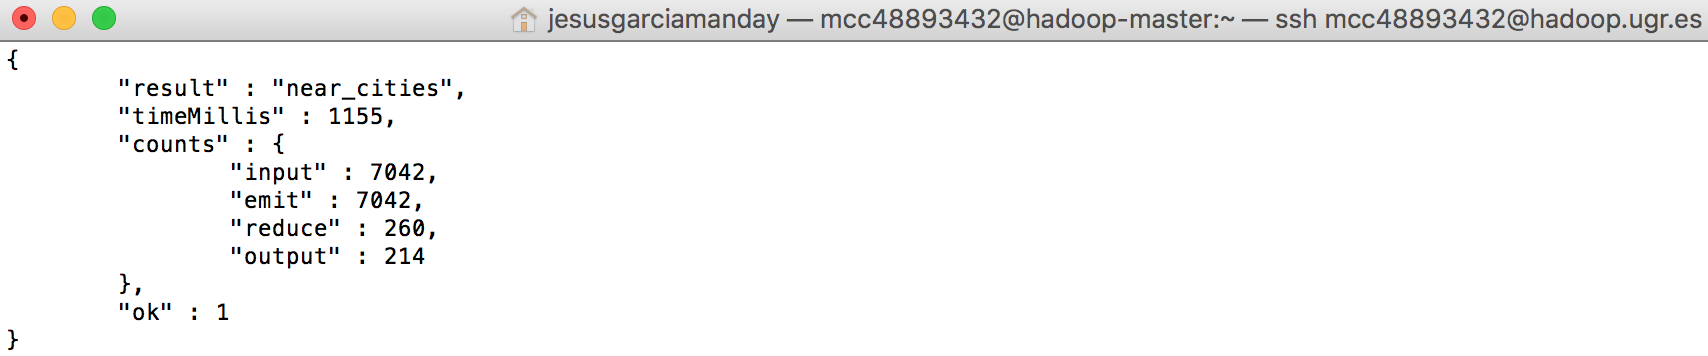
\includegraphics[width = 1.00\textwidth]{p3-img31}
 		\captionof{figure}{\label{fig:IPN}Visualizando los documentos (I).} 
	\end{center} 
\end{figure}

\begin{figure}[H]
	\begin{center}
 		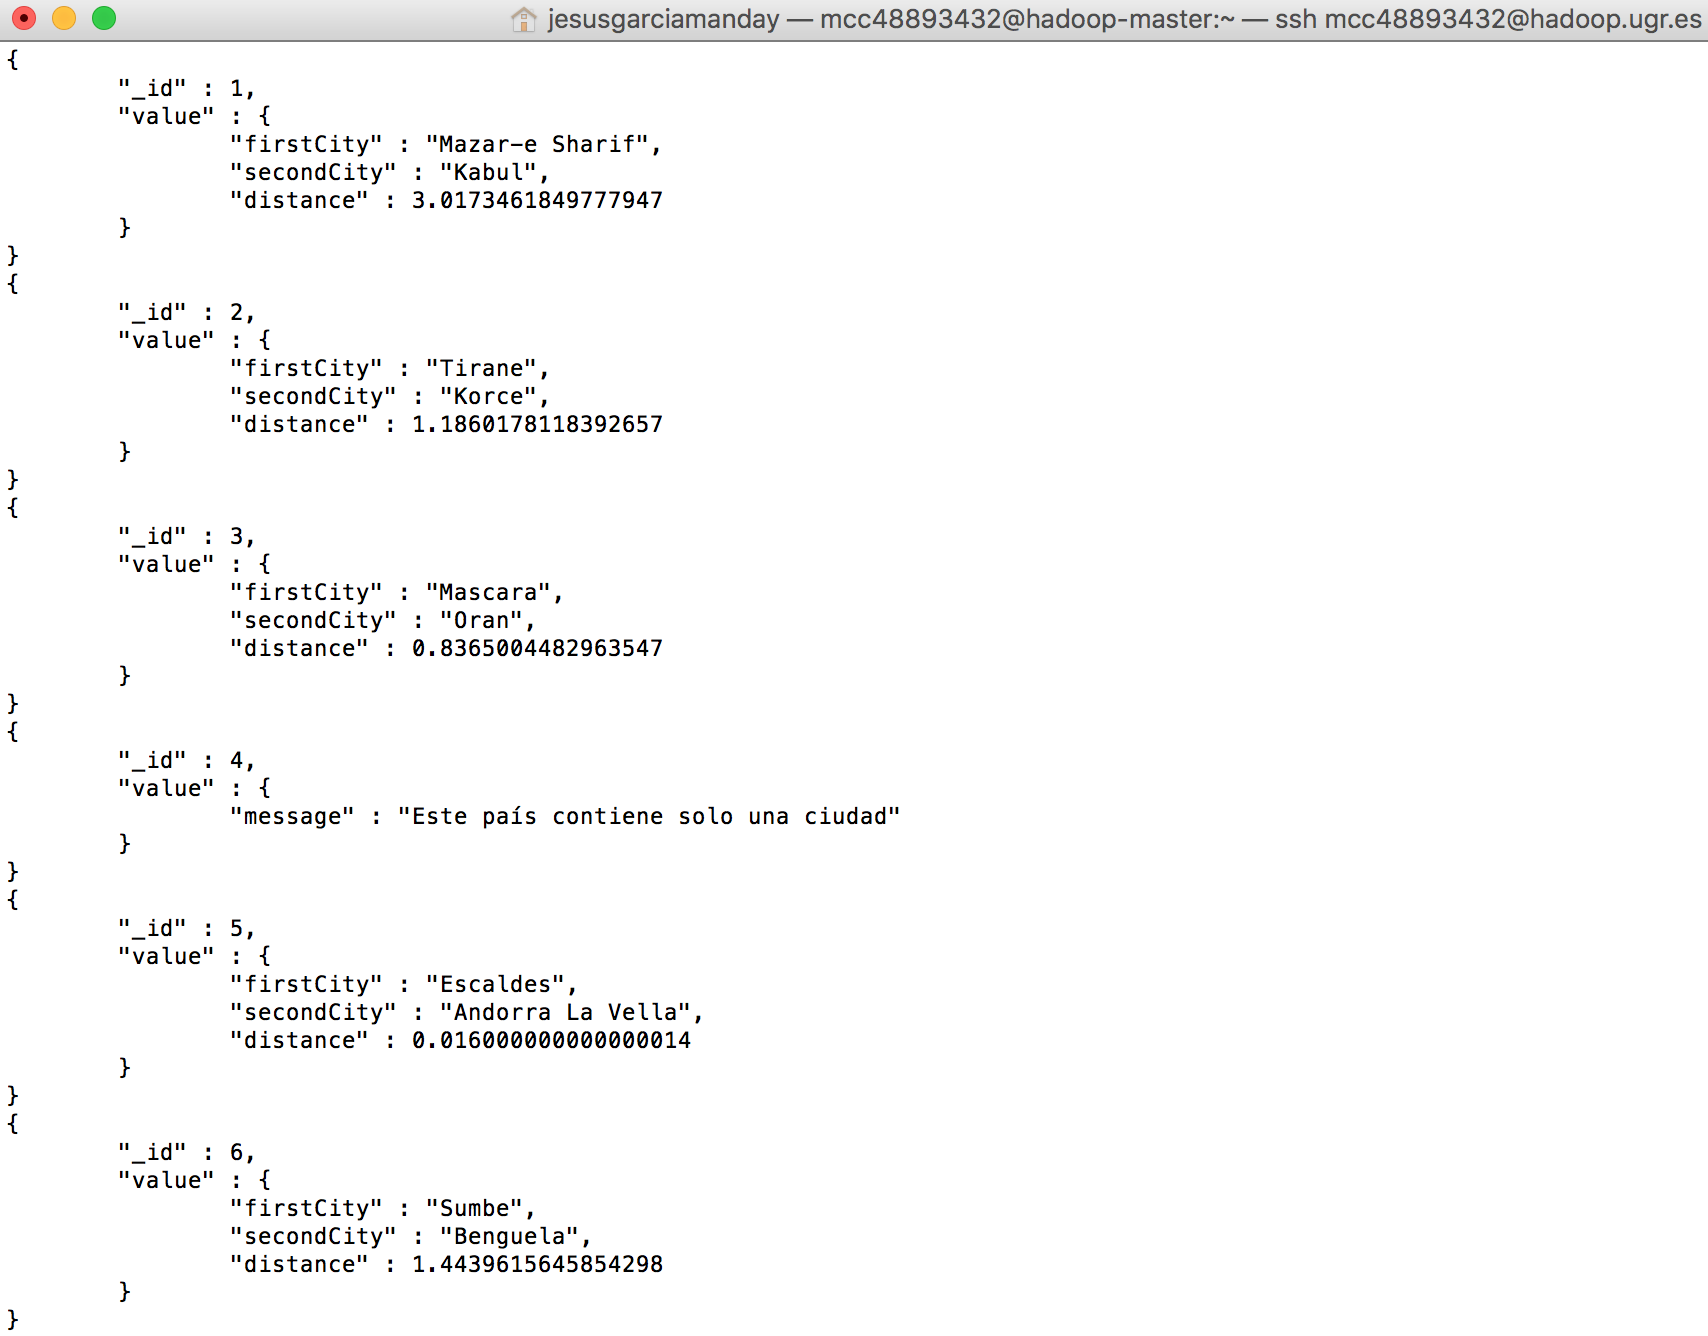
\includegraphics[width = 1.00\textwidth]{p3-img32}
 		\captionof{figure}{\label{fig:IPN}Visualizando los documentos (II).} 
	\end{center} 
\end{figure}

\begin{figure}[H]
	\begin{center}
 		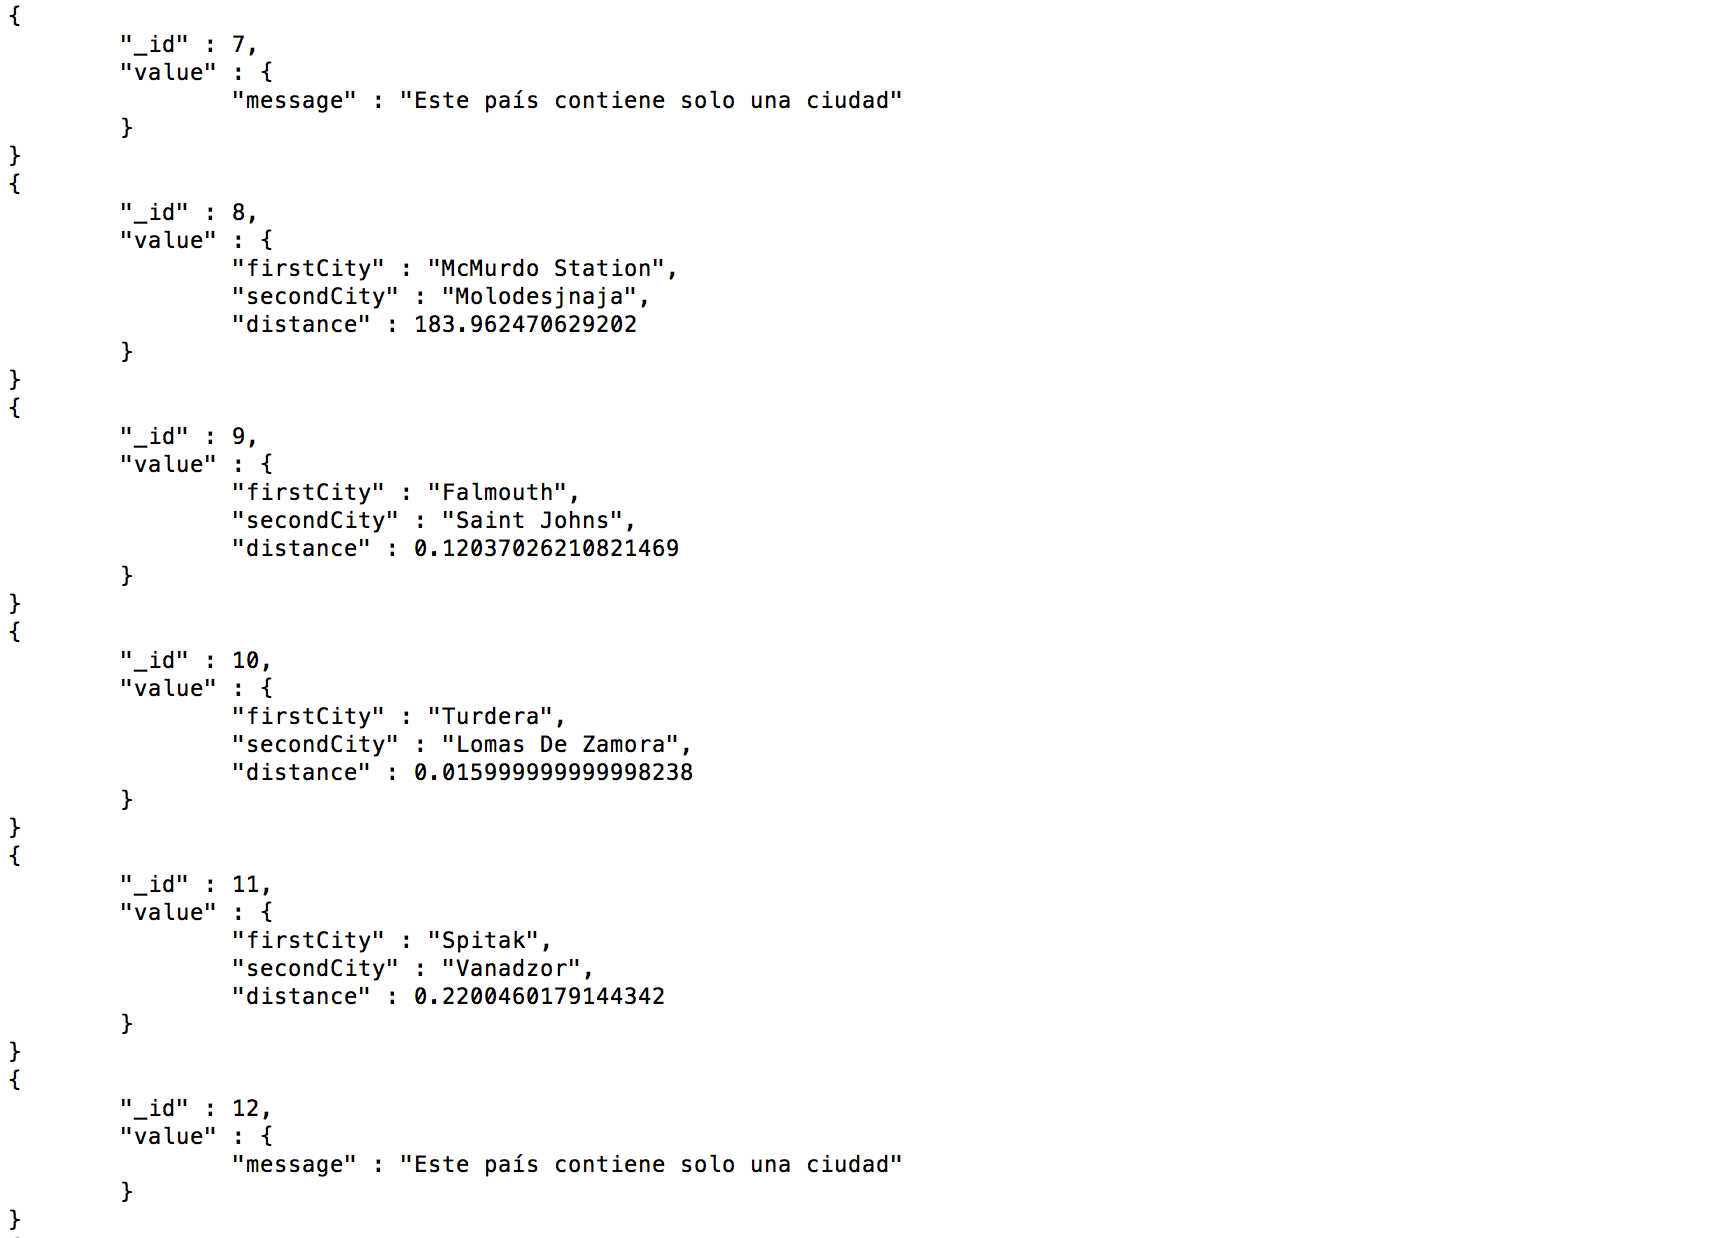
\includegraphics[width = 1.00\textwidth]{p3-img33}
 		\captionof{figure}{\label{fig:IPN}Visualizando los documentos (III).} 
	\end{center} 
\end{figure}

\begin{figure}[H]
	\begin{center}
 		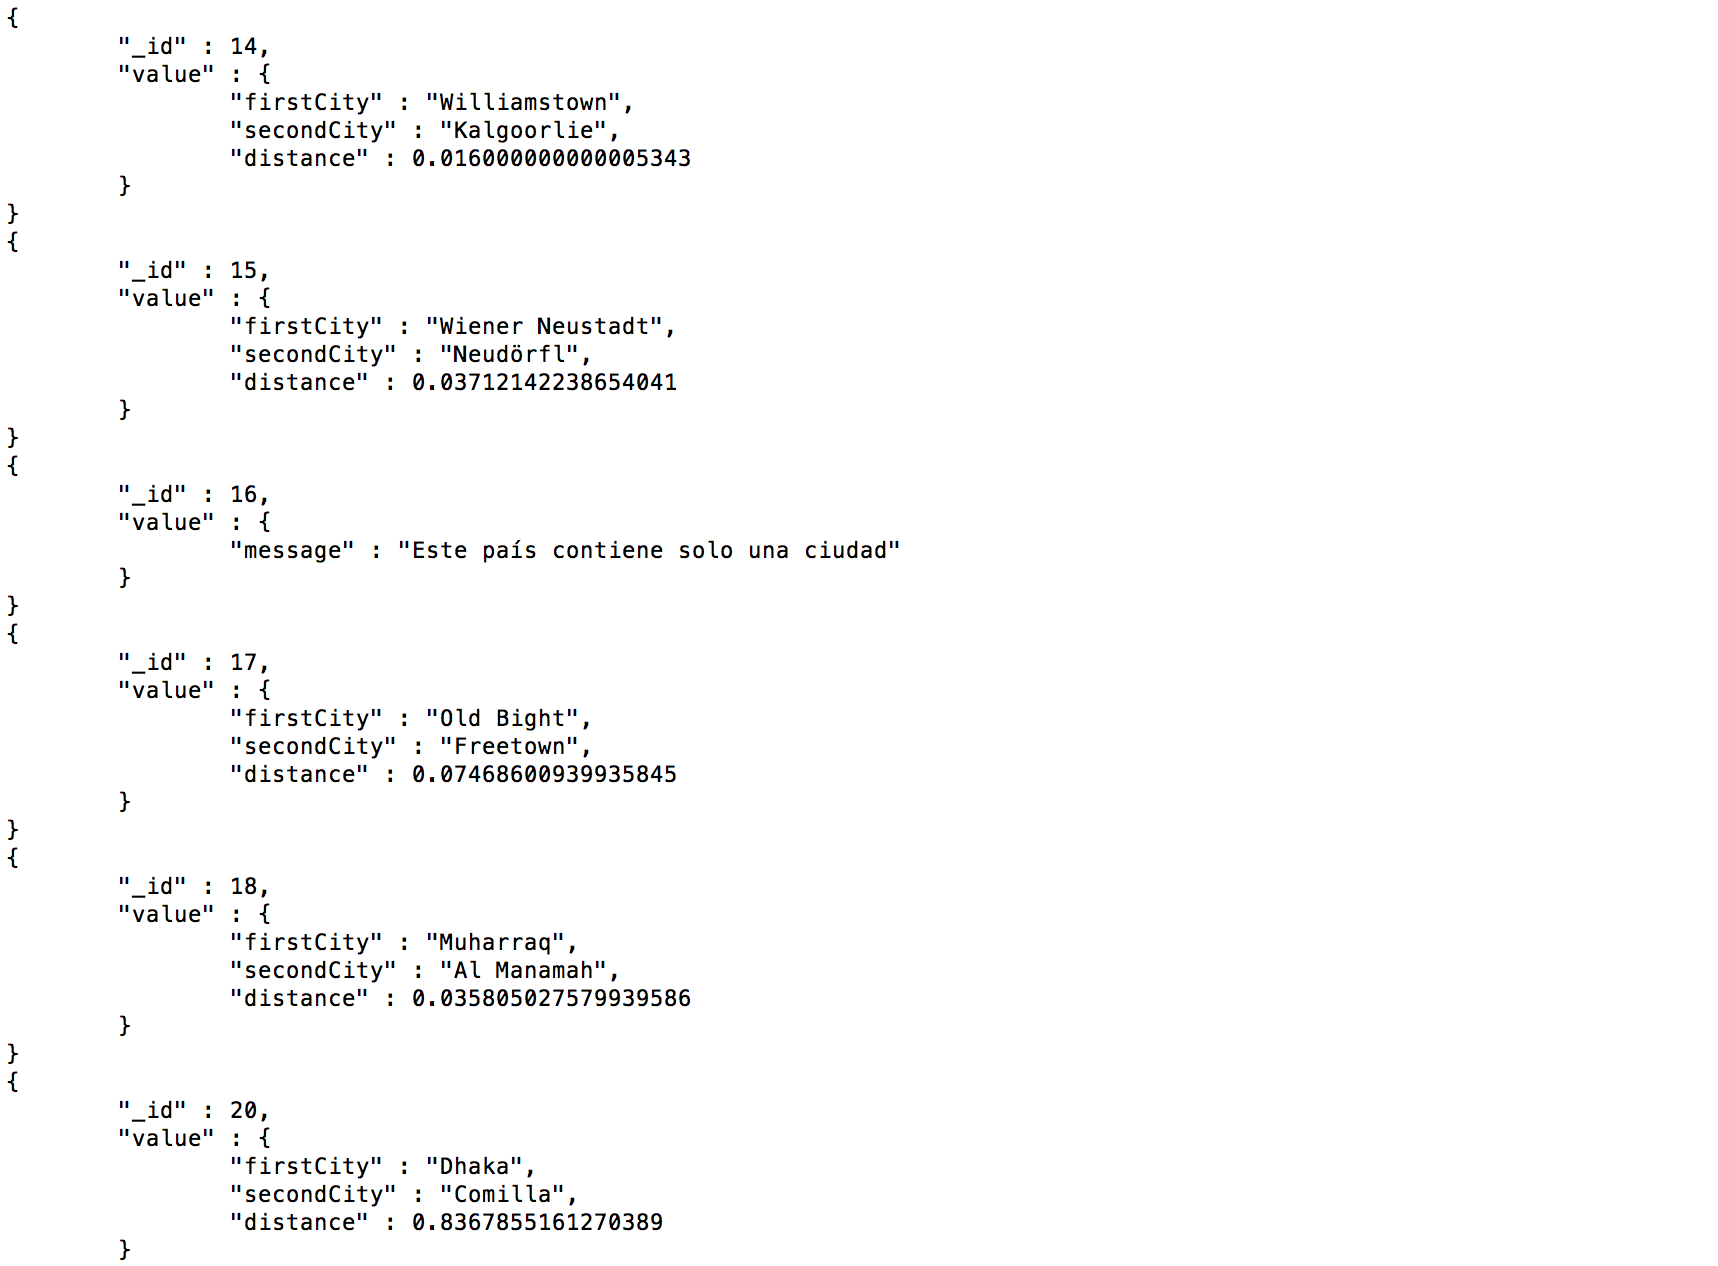
\includegraphics[width = 1.00\textwidth]{p3-img34}
 		\captionof{figure}{\label{fig:IPN}Visualizando los documentos (IV).} 
	\end{center} 
\end{figure}

\begin{figure}[H]
	\begin{center}
 		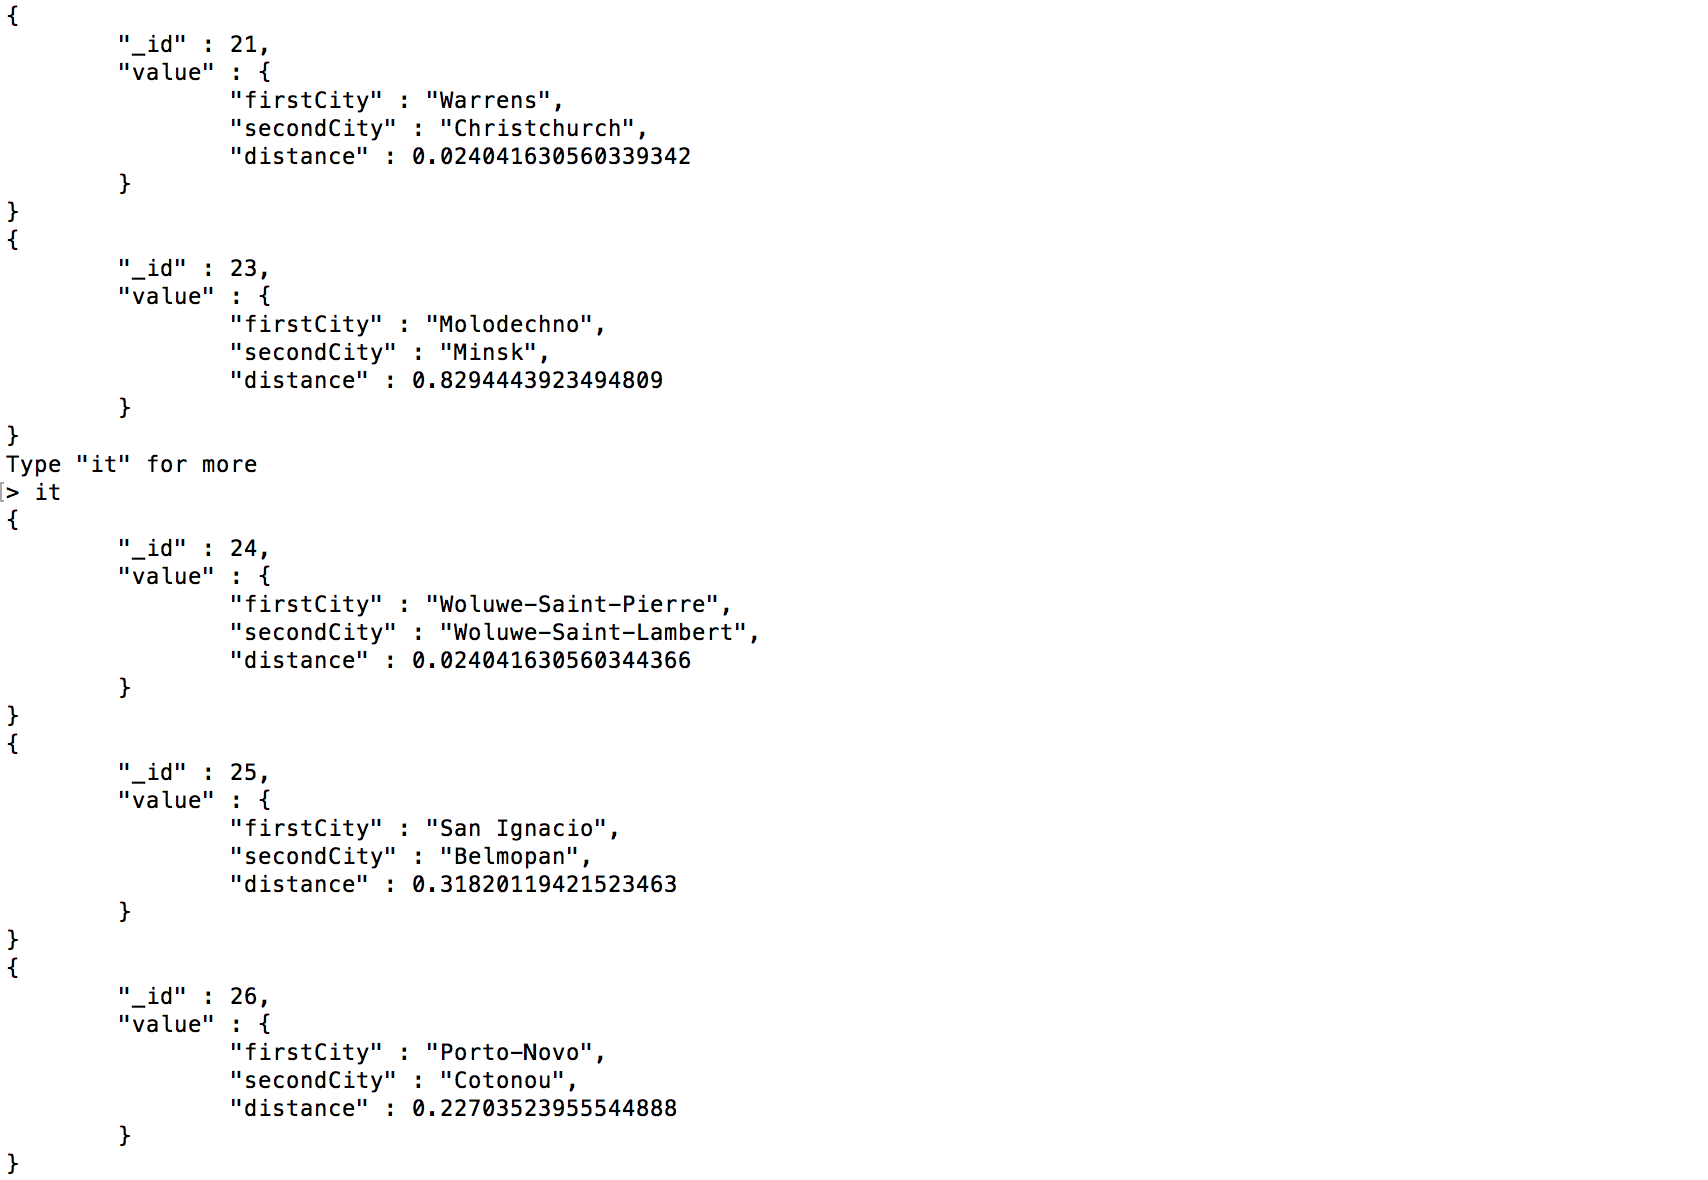
\includegraphics[width = 1.00\textwidth]{p3-img35}
 		\captionof{figure}{\label{fig:IPN}Visualizando los documentos (V).} 
	\end{center} 
\end{figure}

\subsection{¿Cómo podríamos obtener las ciudades más distantes en cada país?.}

\begin{figure}[H]
	\begin{center}
 		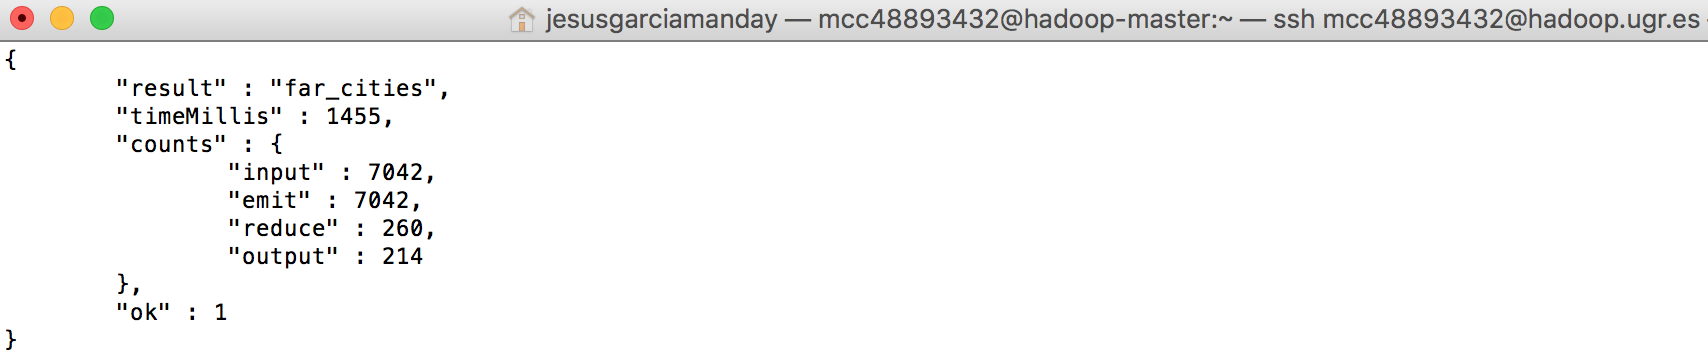
\includegraphics[width = 1.00\textwidth]{p3-img36}
 		\captionof{figure}{\label{fig:IPN}Visualizando los documentos (I).} 
	\end{center} 
\end{figure}

\begin{figure}[H]
	\begin{center}
 		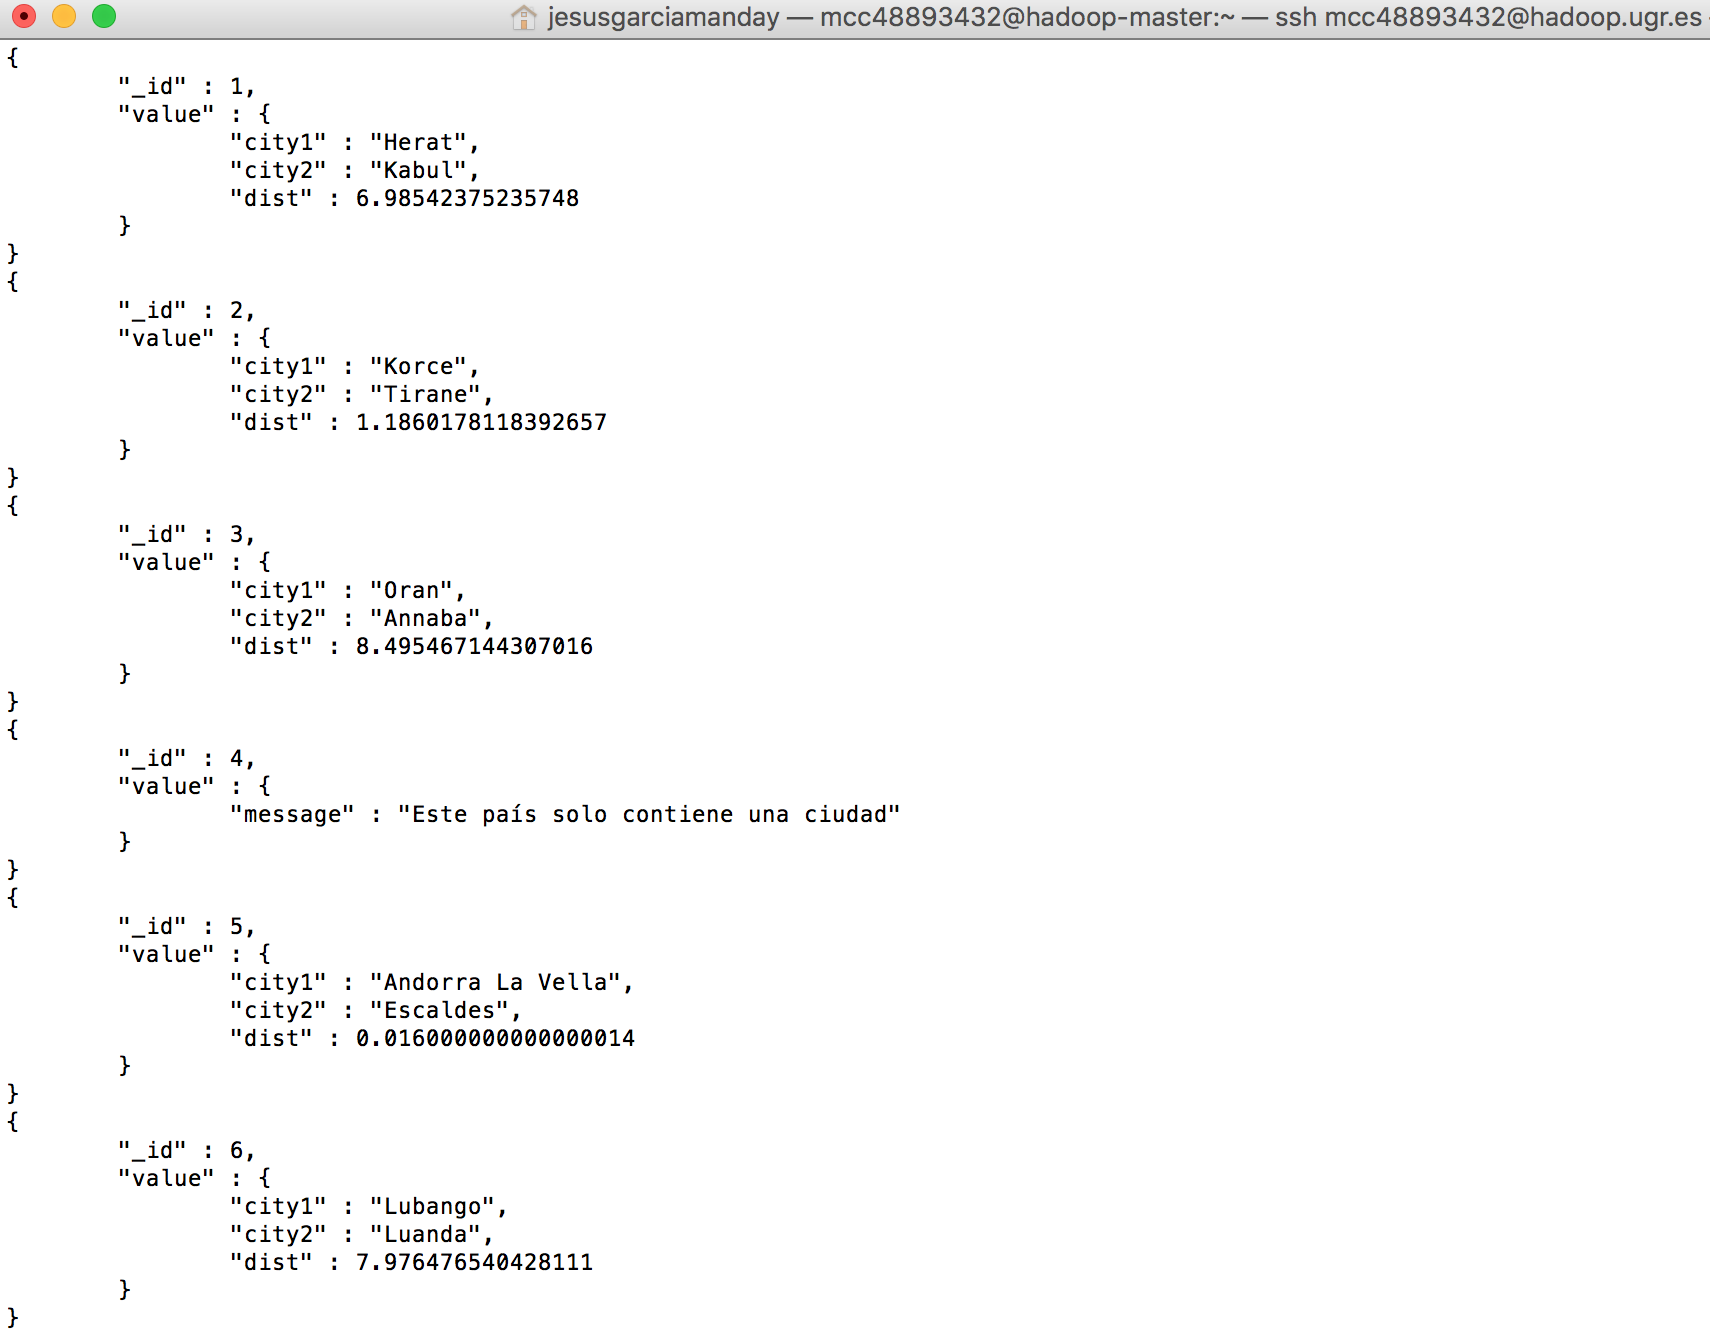
\includegraphics[width = 1.00\textwidth]{p3-img37}
 		\captionof{figure}{\label{fig:IPN}Visualizando los documentos (II).} 
	\end{center} 
\end{figure}

\begin{figure}[H]
	\begin{center}
 		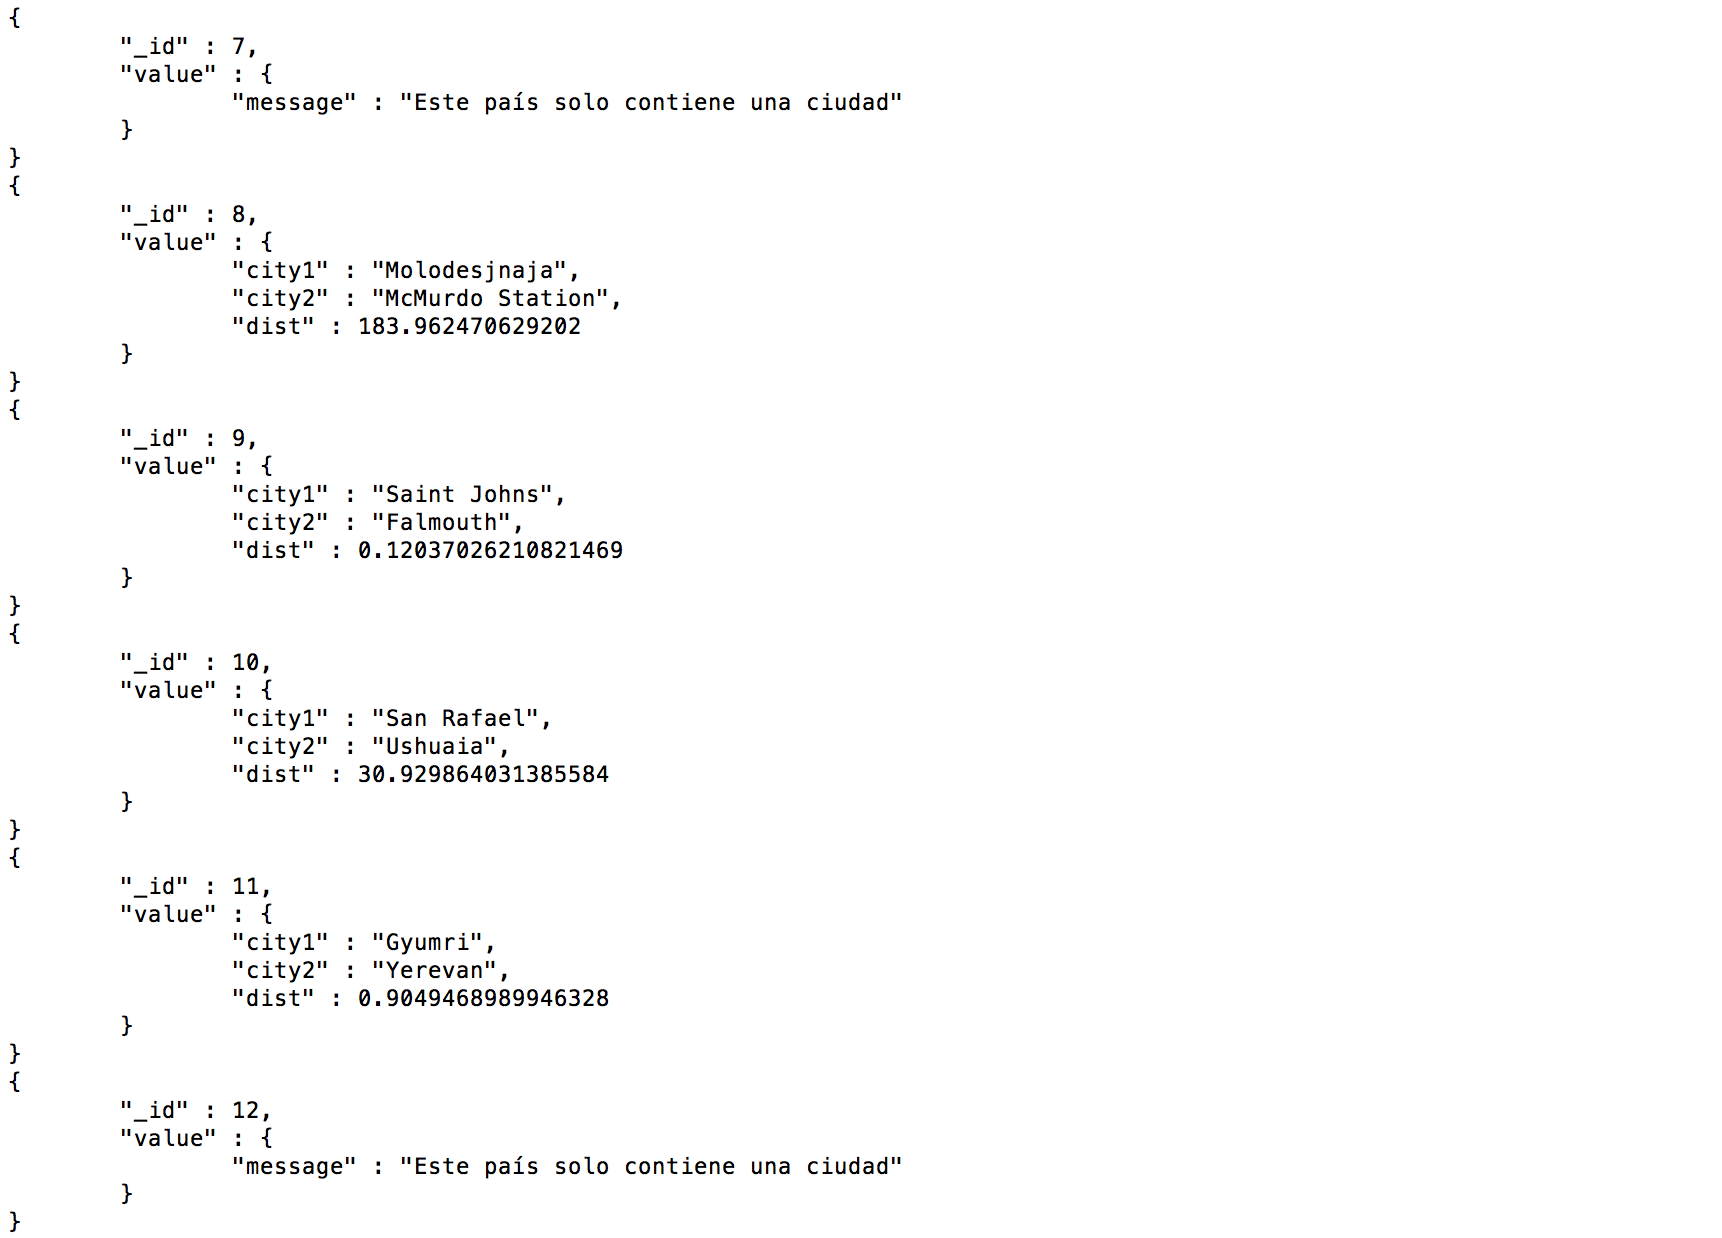
\includegraphics[width = 1.00\textwidth]{p3-img38}
 		\captionof{figure}{\label{fig:IPN}Visualizando los documentos (III).} 
	\end{center} 
\end{figure}

\begin{figure}[H]
	\begin{center}
 		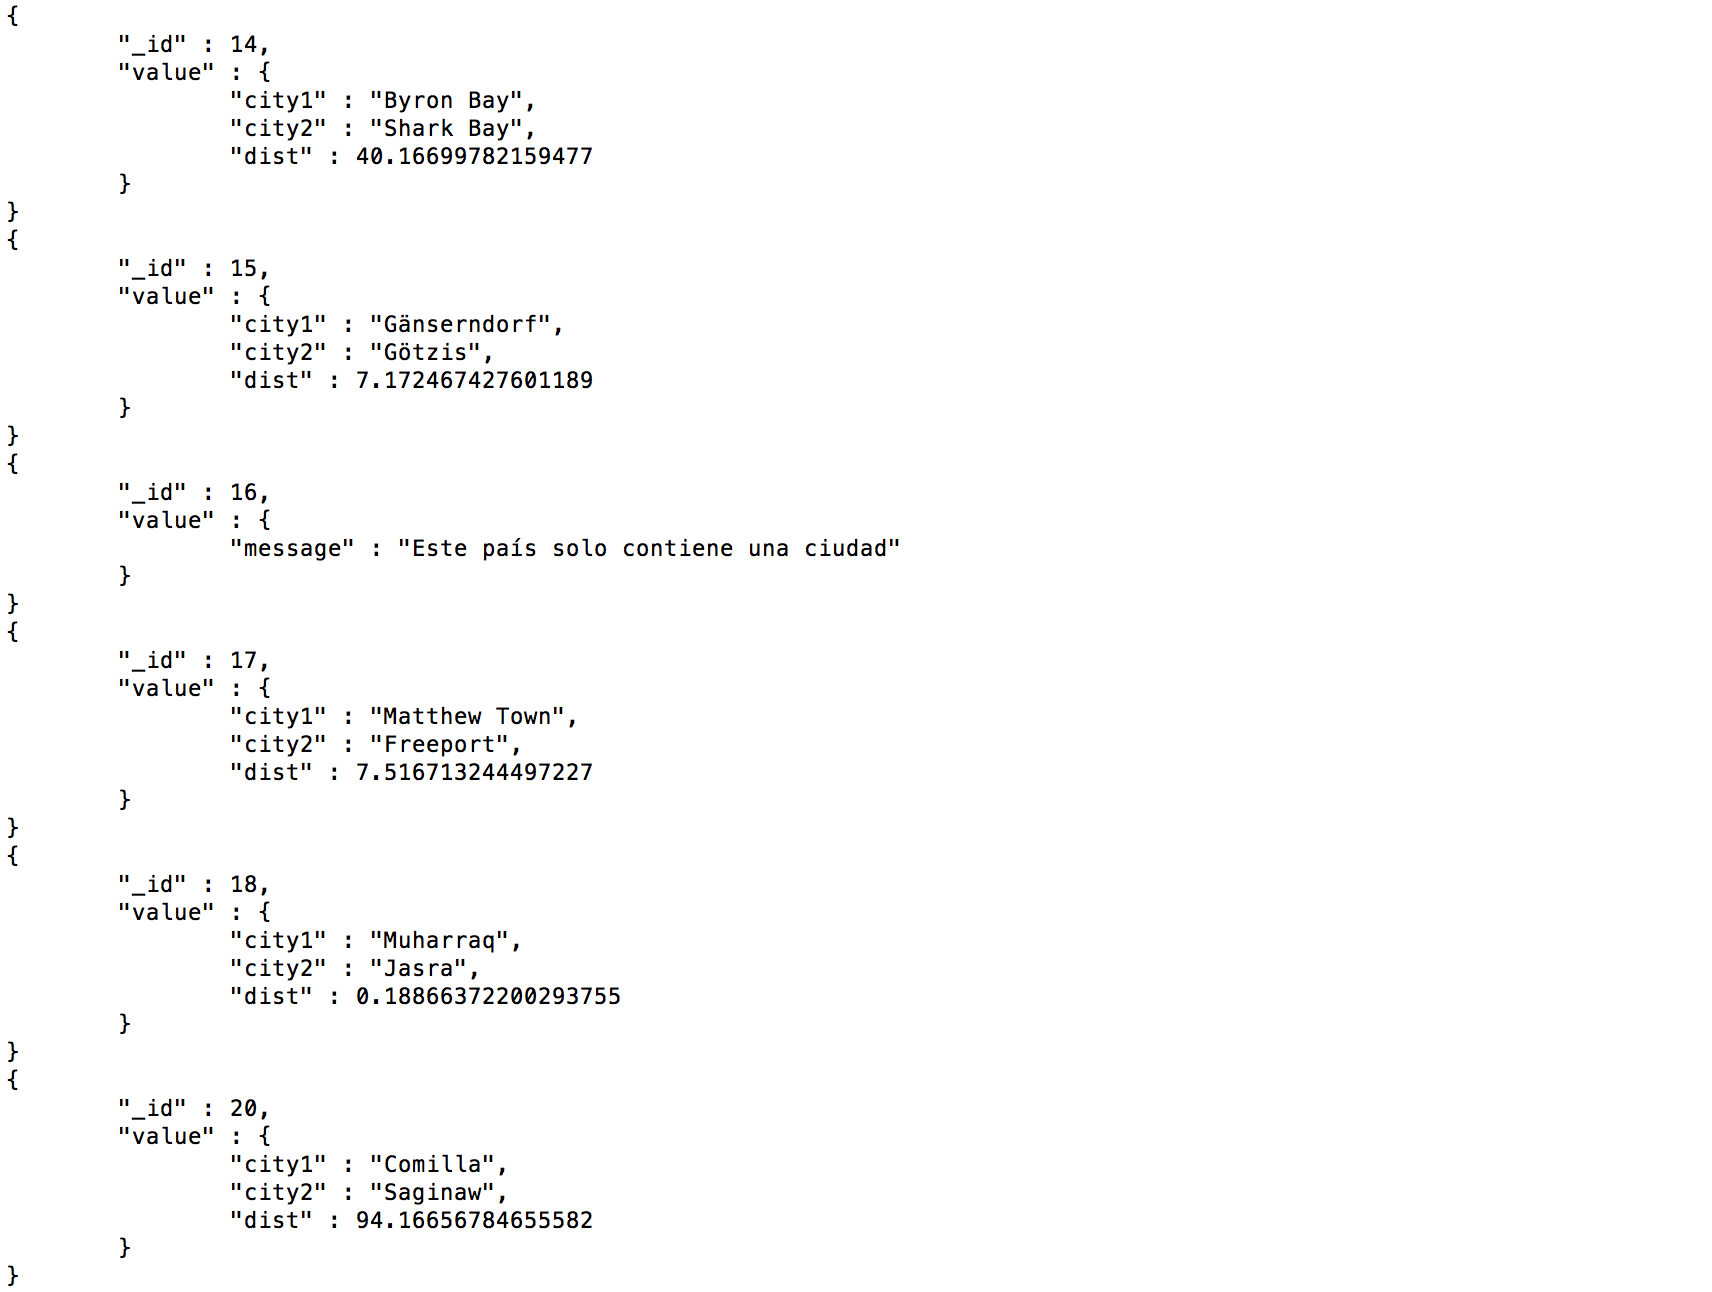
\includegraphics[width = 1.00\textwidth]{p3-img39}
 		\captionof{figure}{\label{fig:IPN}Visualizando los documentos (IV).} 
	\end{center} 
\end{figure}

\begin{figure}[H]
	\begin{center}
 		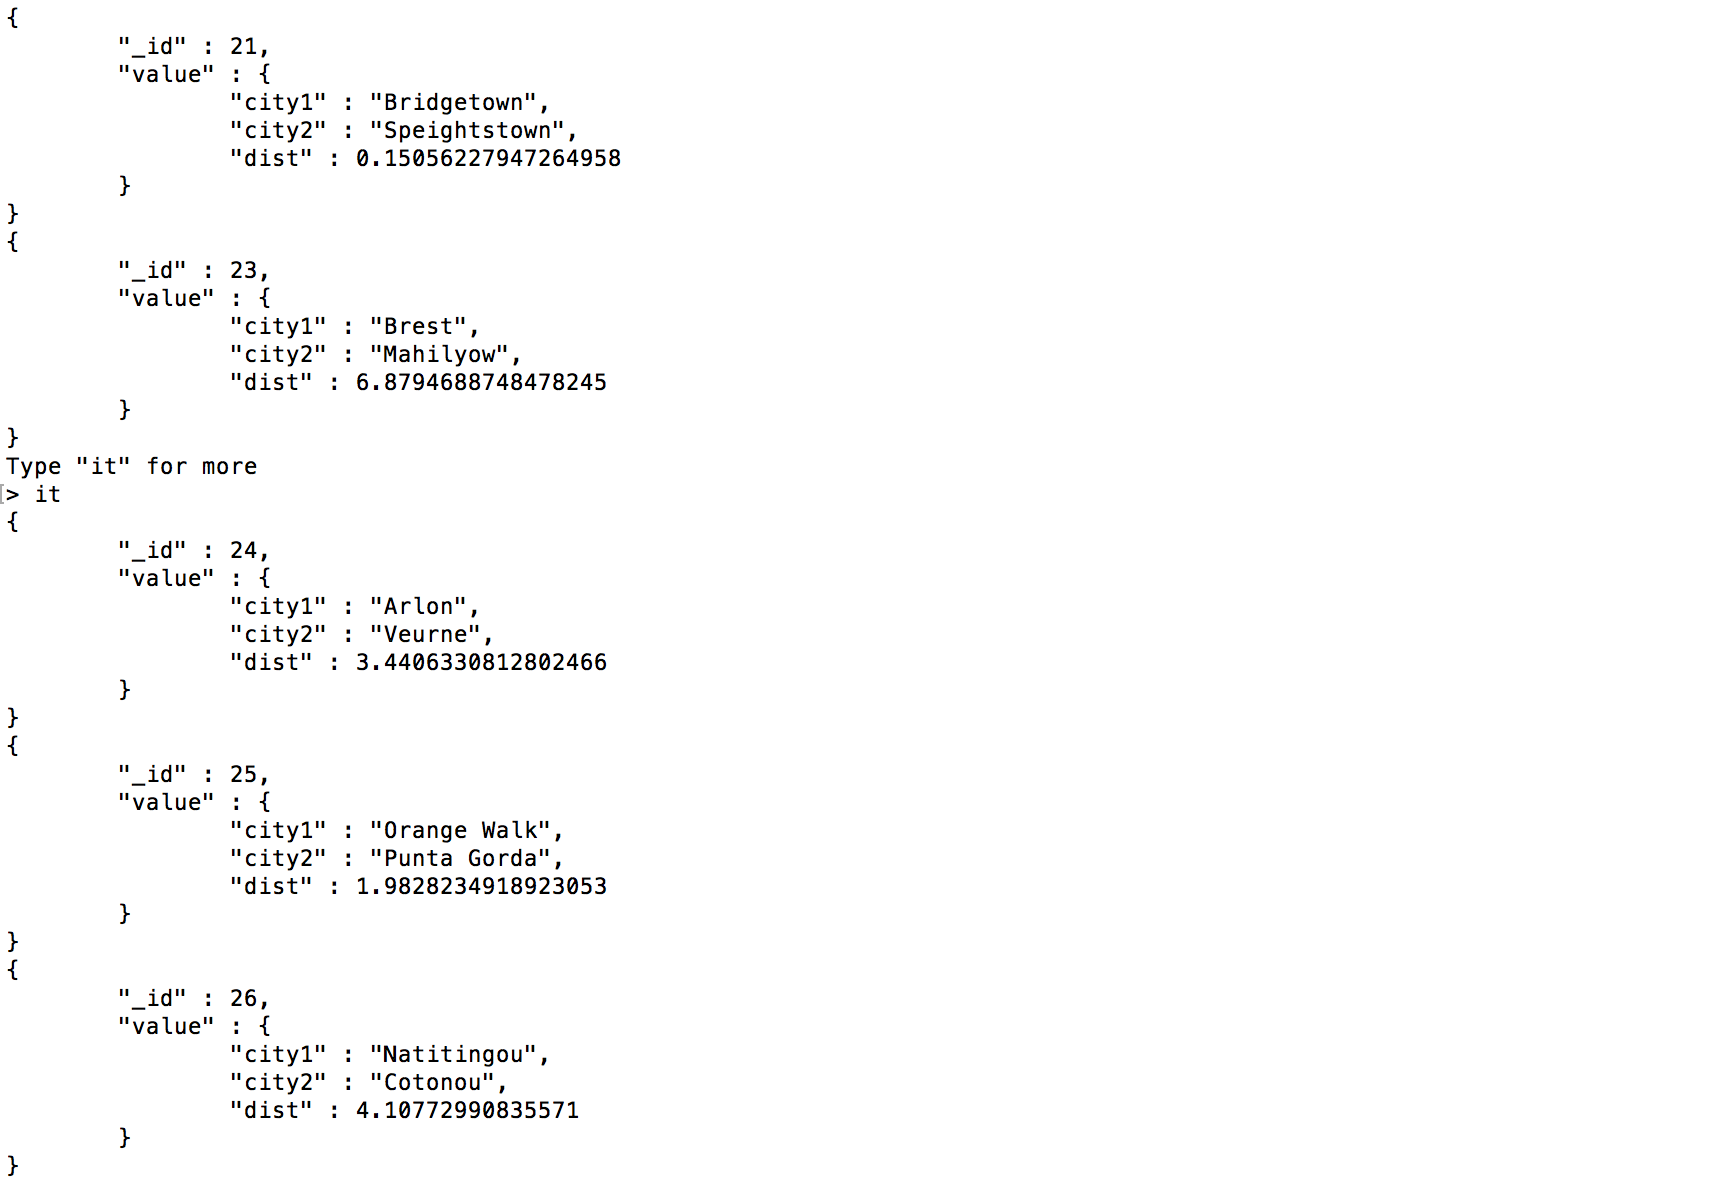
\includegraphics[width = 1.00\textwidth]{p3-img40}
 		\captionof{figure}{\label{fig:IPN}Visualizando los documentos (V).} 
	\end{center} 
\end{figure}


\subsection{¿Qué ocurre si en un país hay dos parejas de ciudades que están a la misma distancia mínima?¿Cómo harías para que aparecieran todas?.}

\begin{figure}[H]
	\begin{center}
 		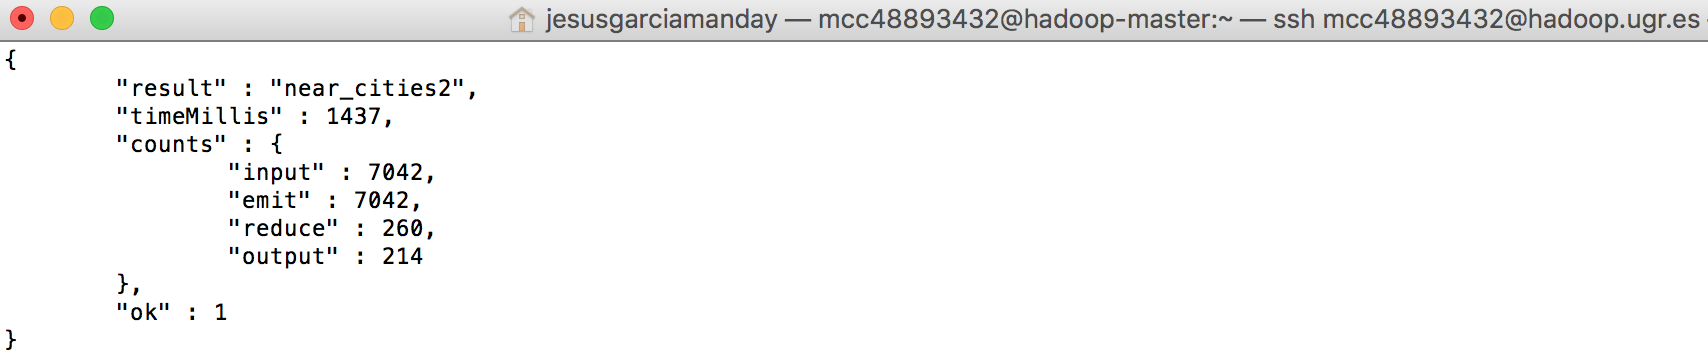
\includegraphics[width = 1.00\textwidth]{p3-img41}
 		\captionof{figure}{\label{fig:IPN}Visualizando los documentos (I).} 
	\end{center} 
\end{figure}

\begin{figure}[H]
	\begin{center}
 		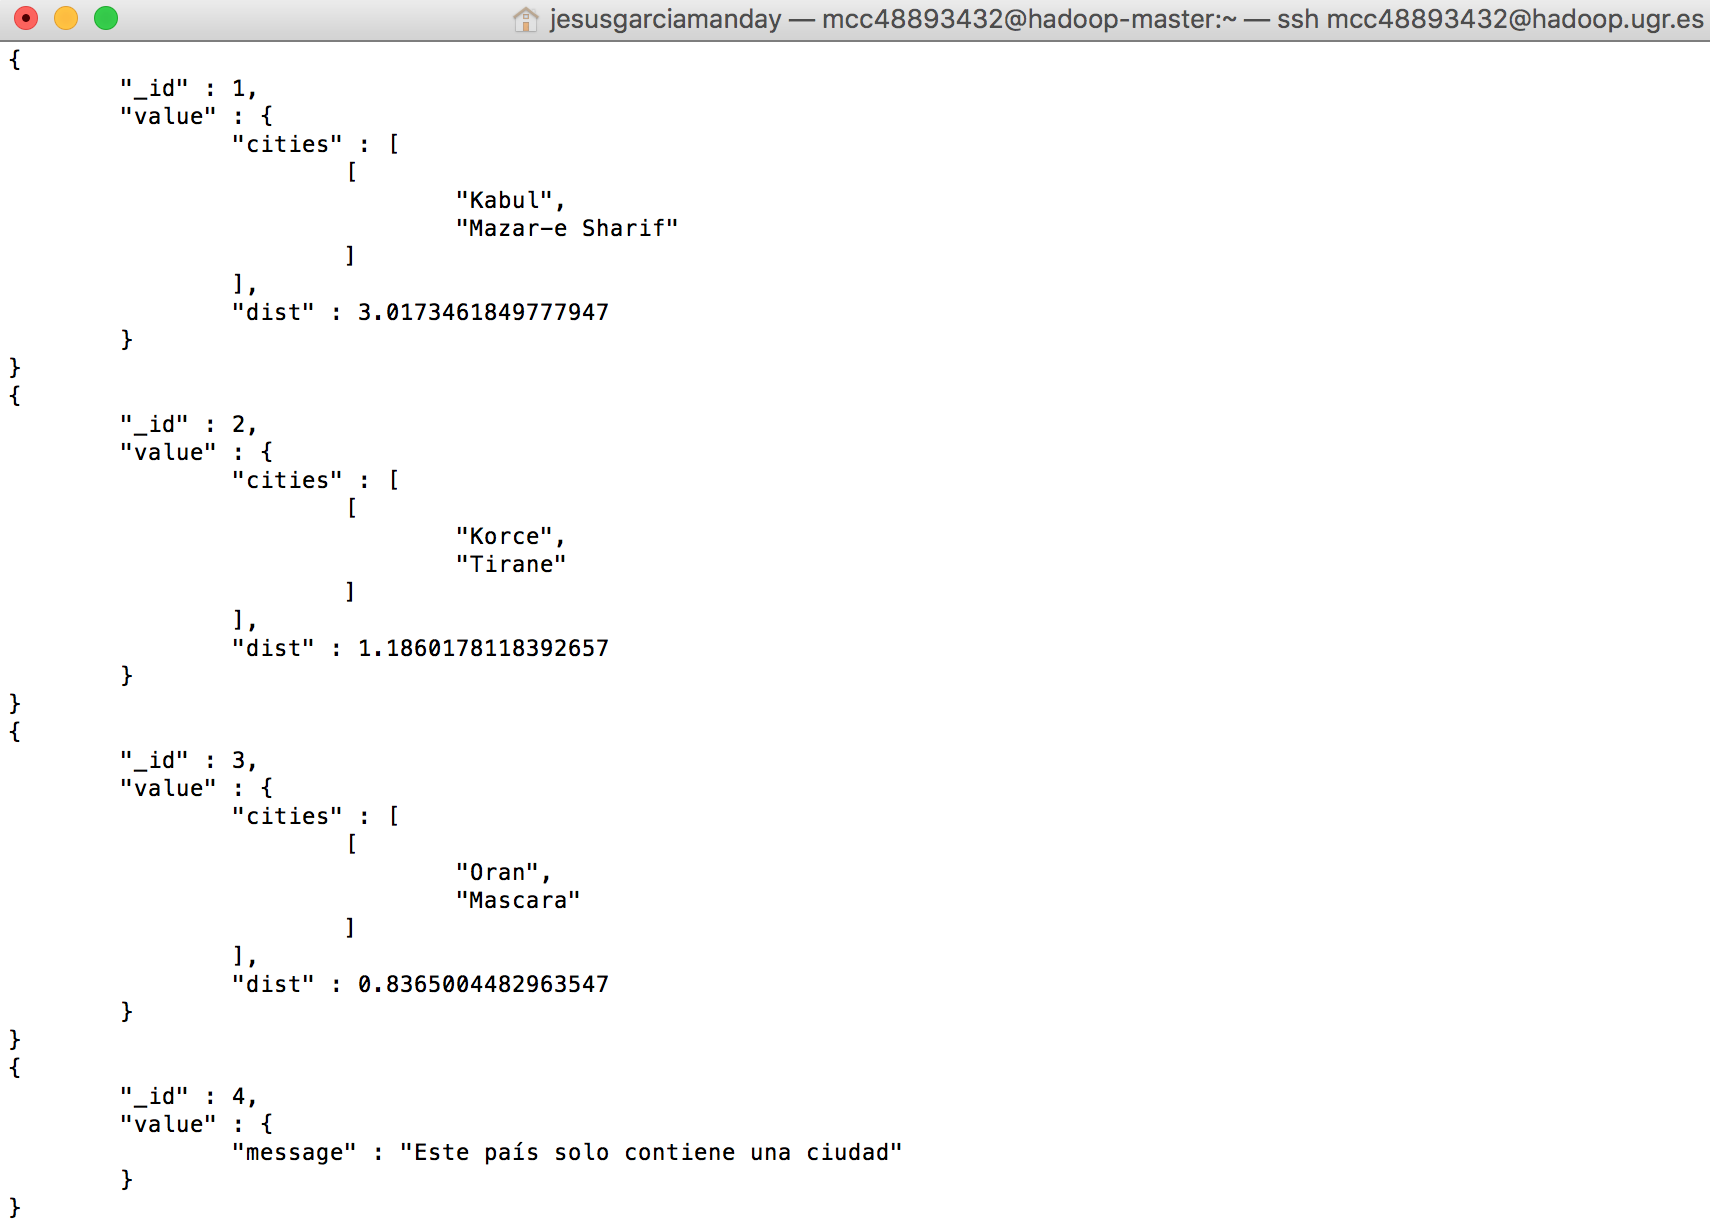
\includegraphics[width = 1.00\textwidth]{p3-img42}
 		\captionof{figure}{\label{fig:IPN}Visualizando los documentos (II).} 
	\end{center} 
\end{figure}

\begin{figure}[H]
	\begin{center}
 		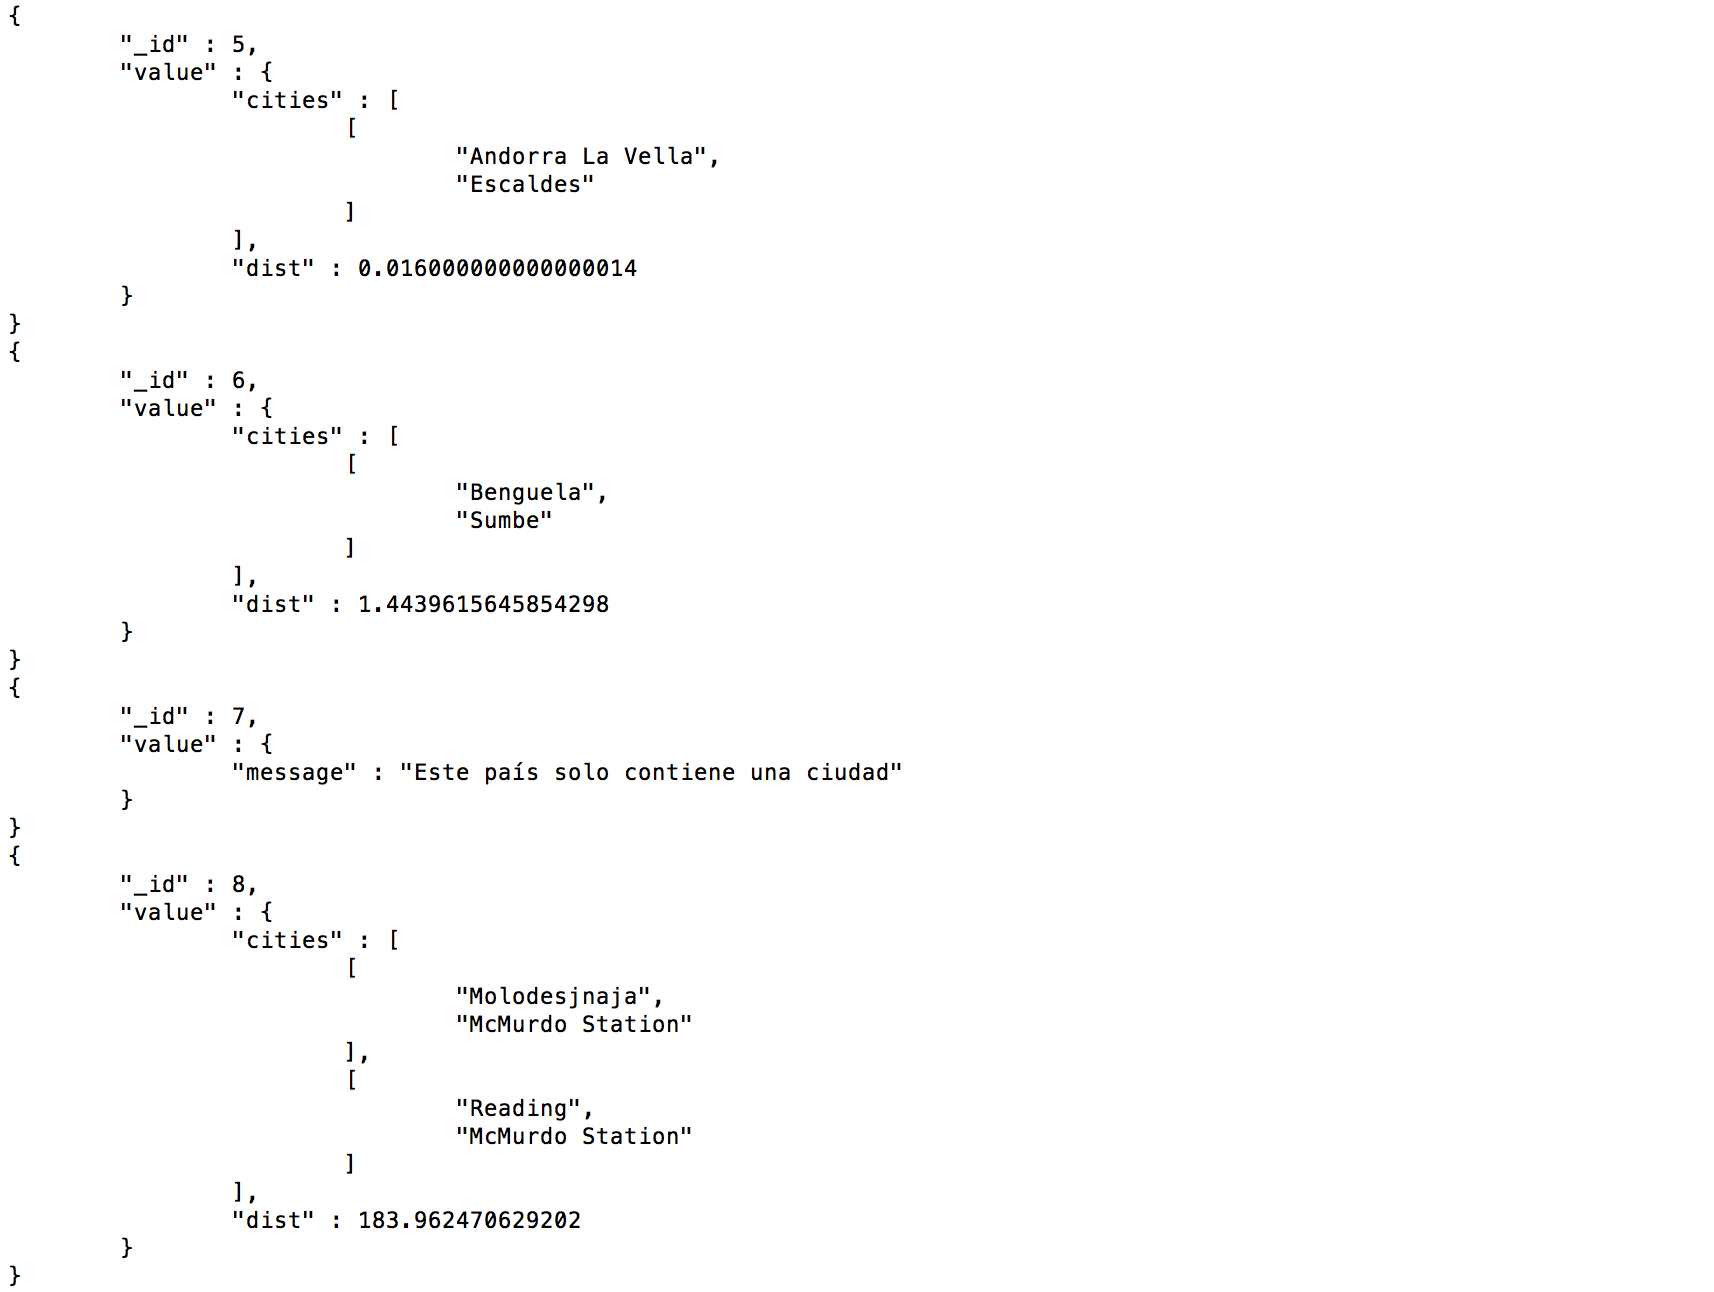
\includegraphics[width = 1.00\textwidth]{p3-img43}
 		\captionof{figure}{\label{fig:IPN}Visualizando los documentos (III).} 
	\end{center} 
\end{figure}

\begin{figure}[H]
	\begin{center}
 		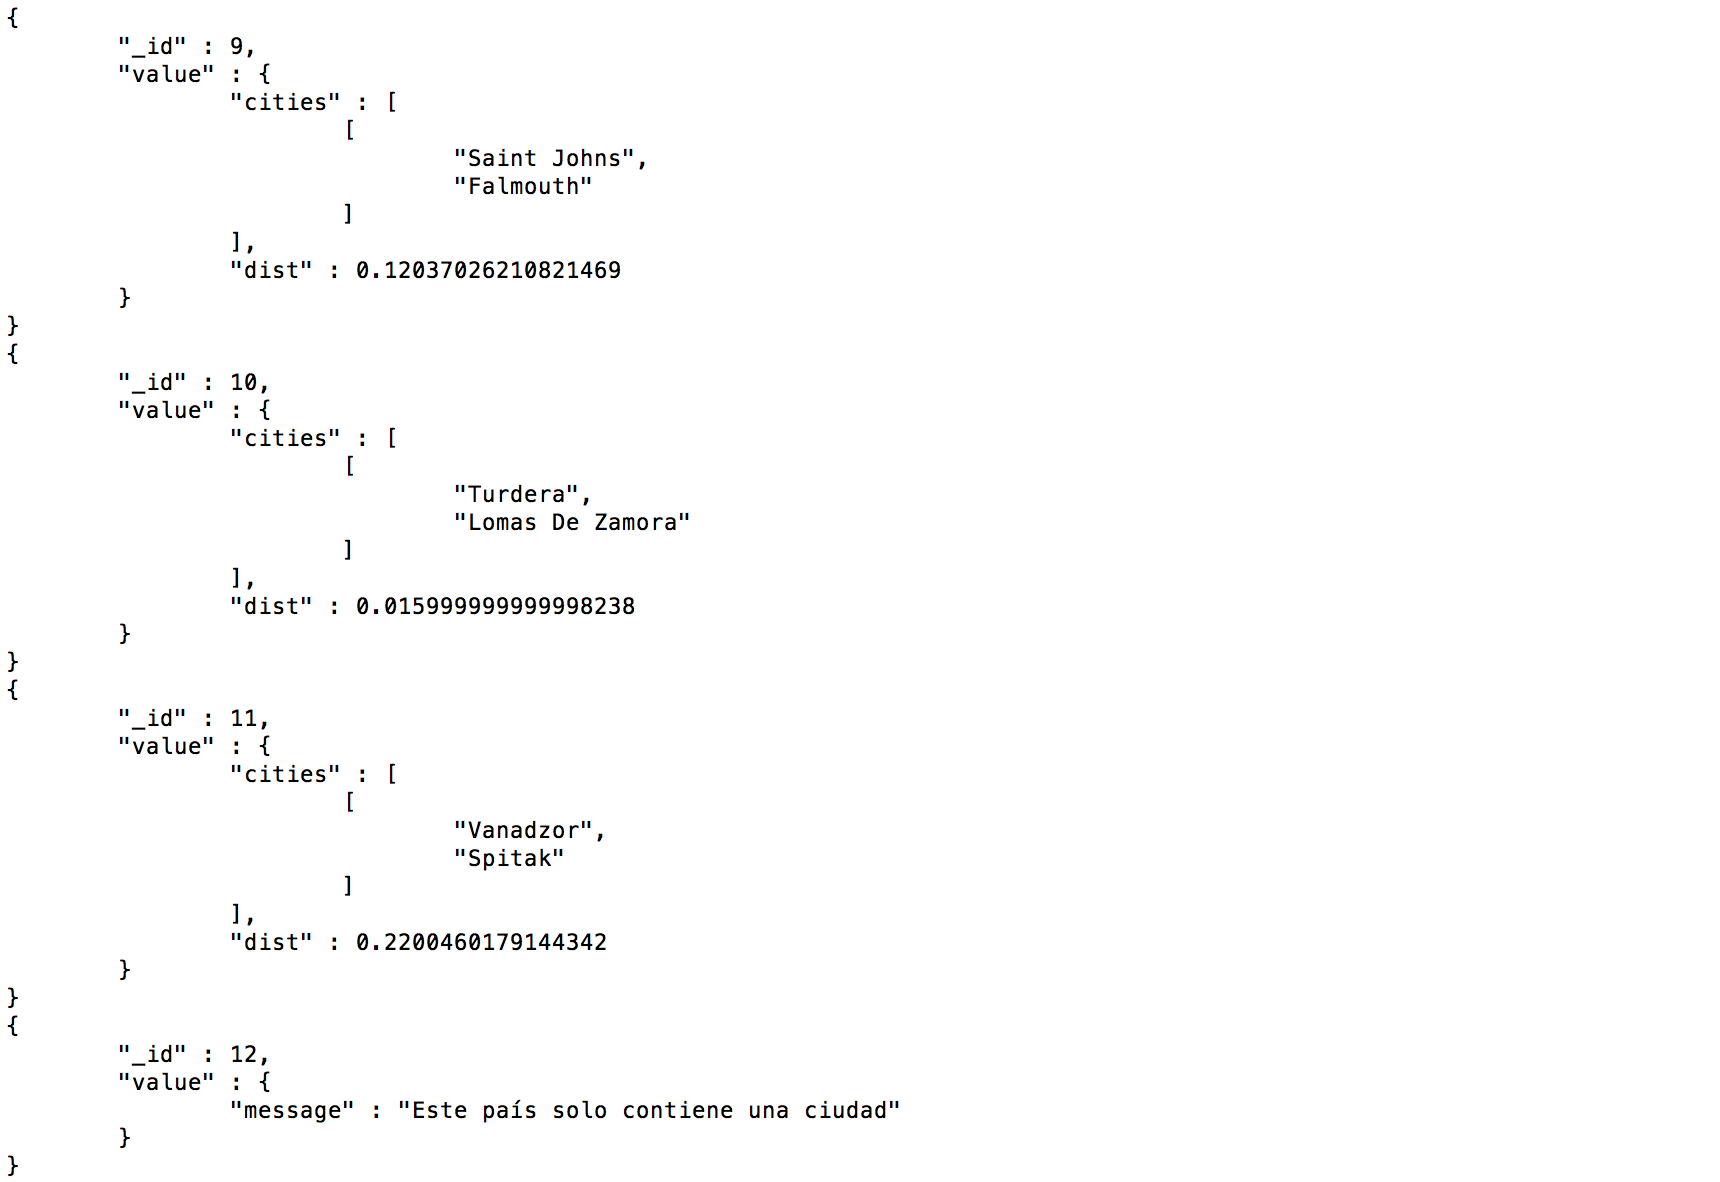
\includegraphics[width = 1.00\textwidth]{p3-img44}
 		\captionof{figure}{\label{fig:IPN}Visualizando los documentos (IV).} 
	\end{center} 
\end{figure}

\begin{figure}[H]
	\begin{center}
 		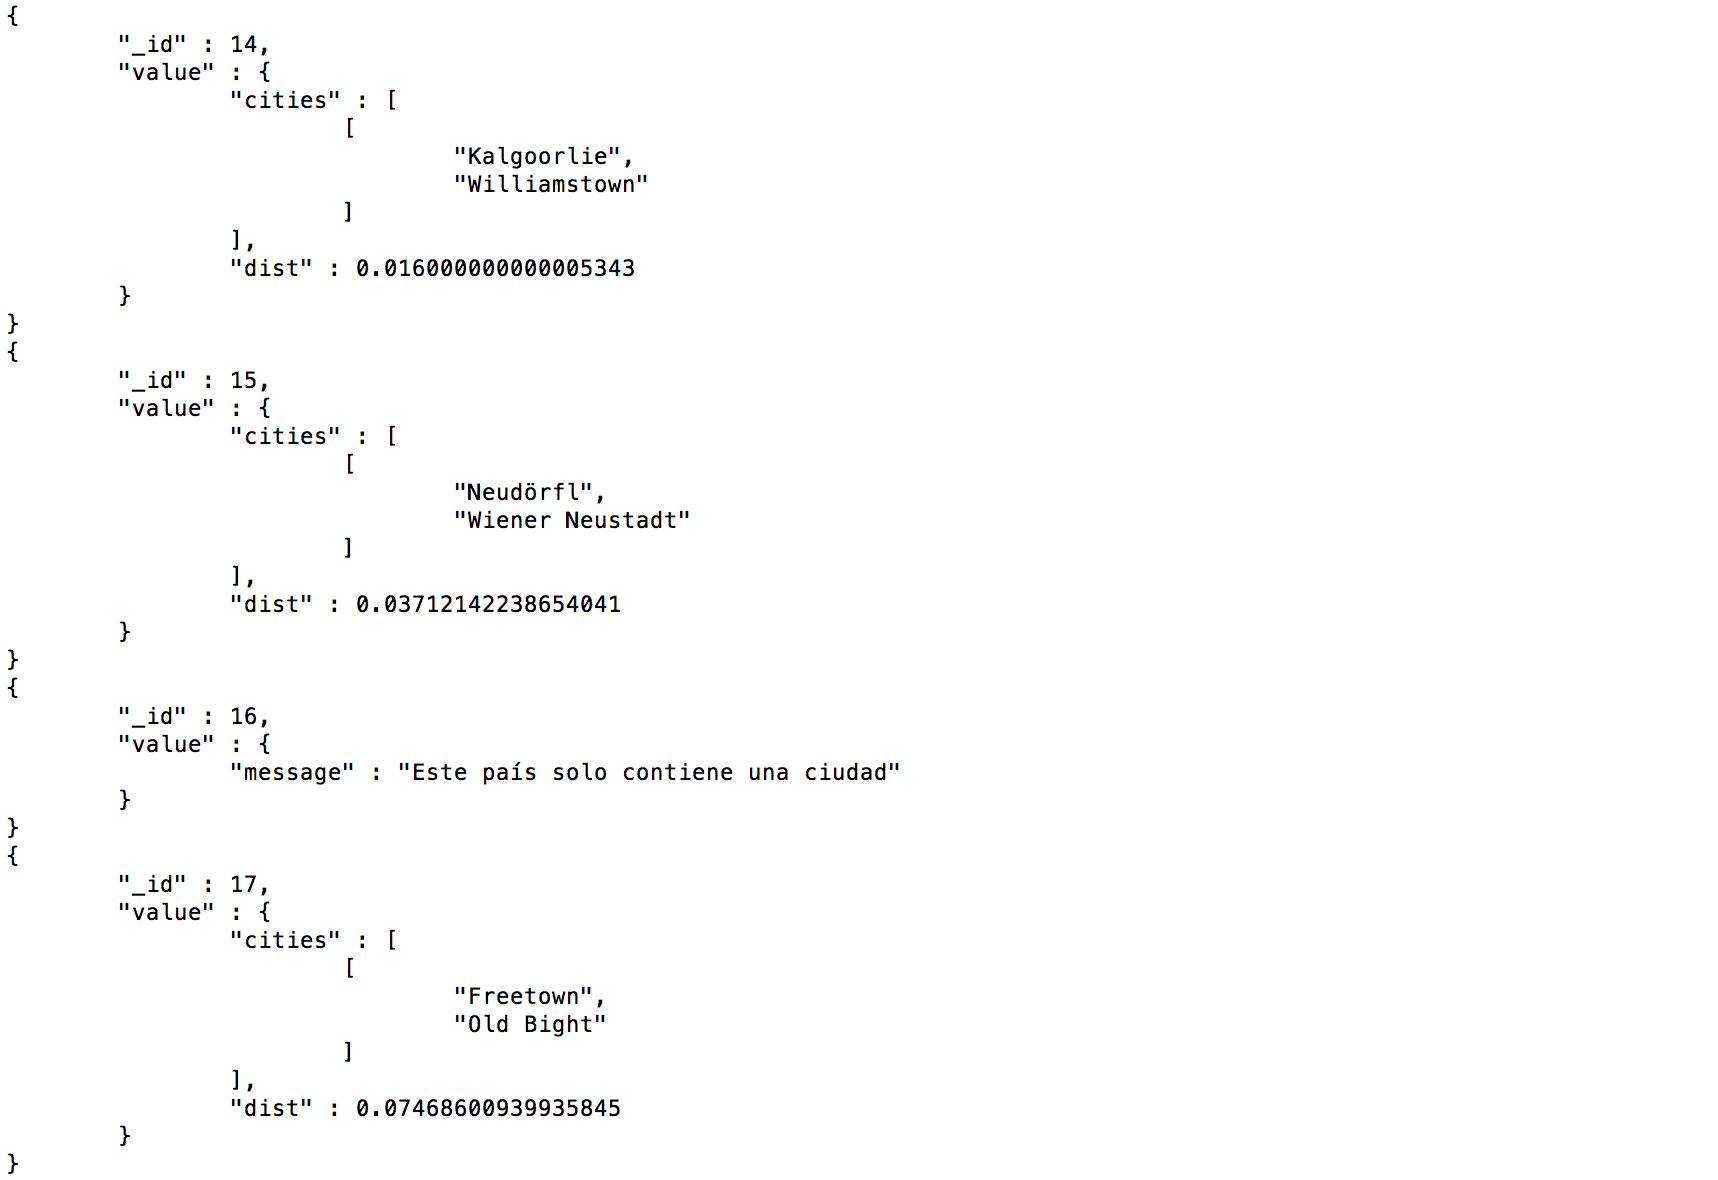
\includegraphics[width = 1.00\textwidth]{p3-img45}
 		\captionof{figure}{\label{fig:IPN}Visualizando los documentos (V).} 
	\end{center} 
\end{figure}

\begin{figure}[H]
	\begin{center}
 		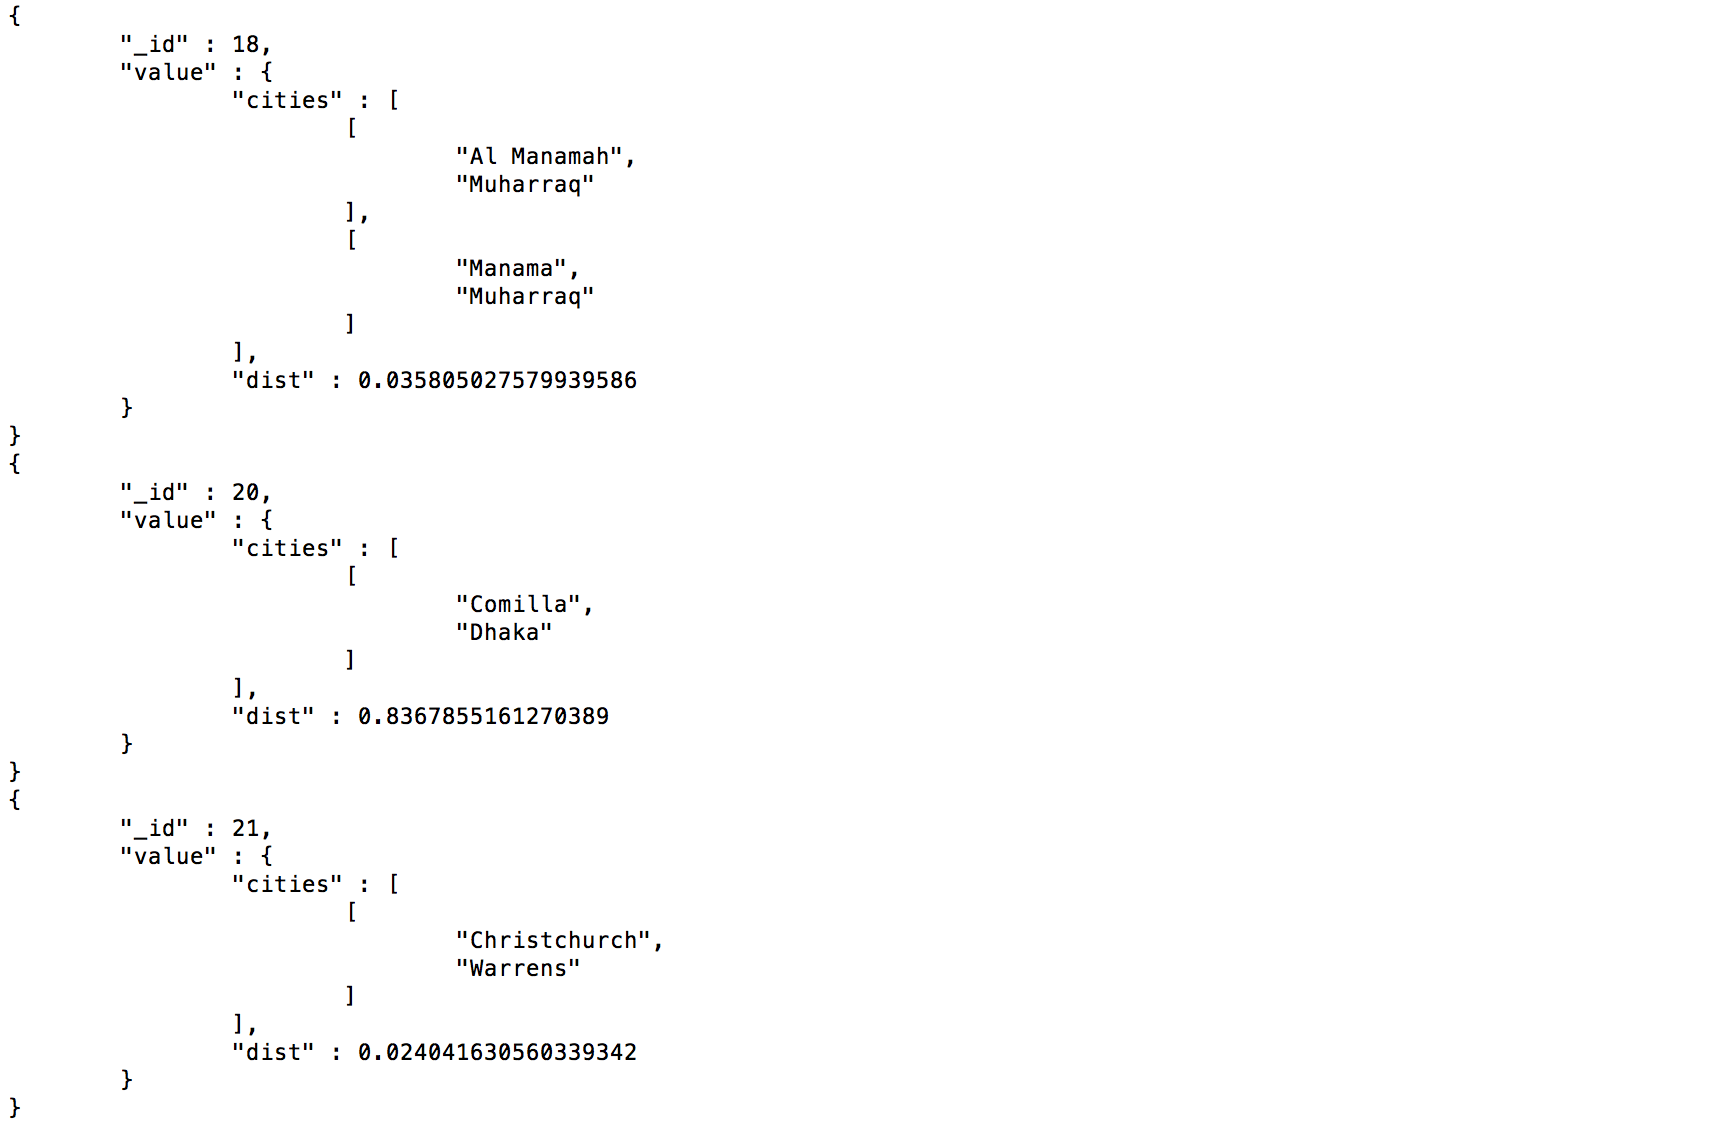
\includegraphics[width = 1.00\textwidth]{p3-img46}
 		\captionof{figure}{\label{fig:IPN}Visualizando los documentos (VI).} 
	\end{center} 
\end{figure}

\begin{figure}[H]
	\begin{center}
 		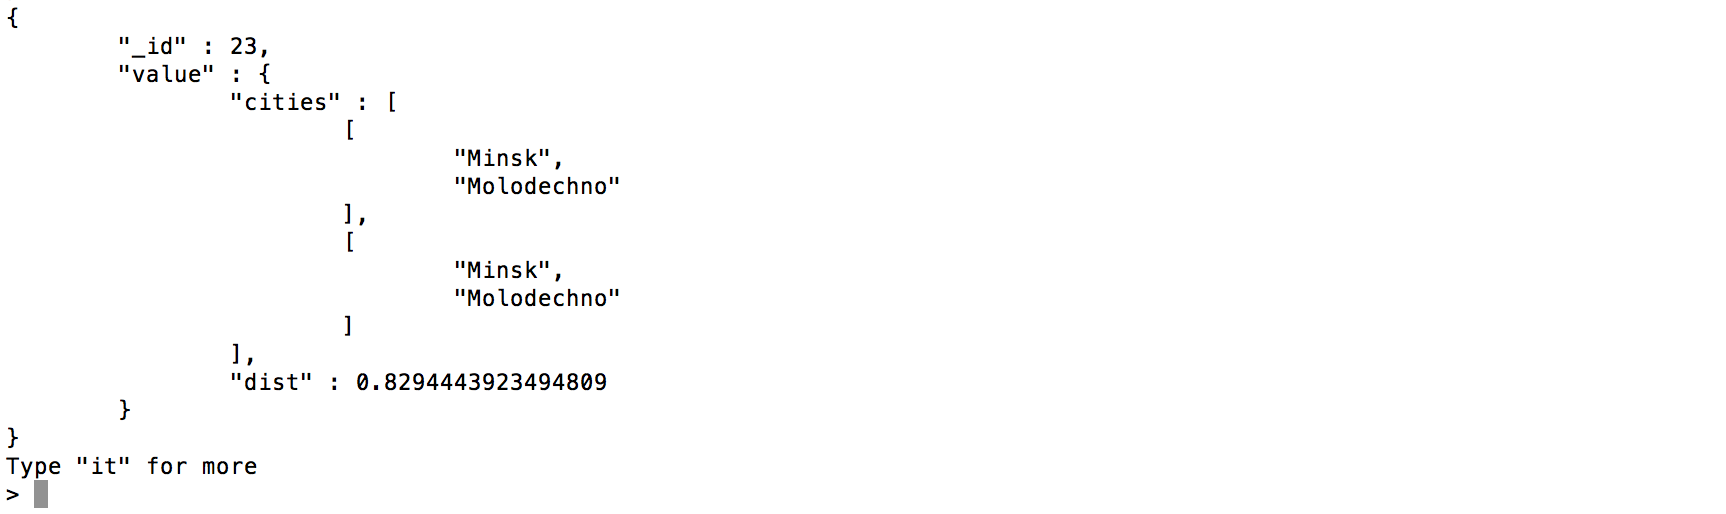
\includegraphics[width = 1.00\textwidth]{p3-img47}
 		\captionof{figure}{\label{fig:IPN}Visualizando los documentos (VII).} 
	\end{center} 
\end{figure}


\subsection{¿Cómo podríamos obtener adicionalmente la cantidad de parejas de ciudades evaluadas para cada país consultado?.}

\begin{figure}[H]
	\begin{center}
 		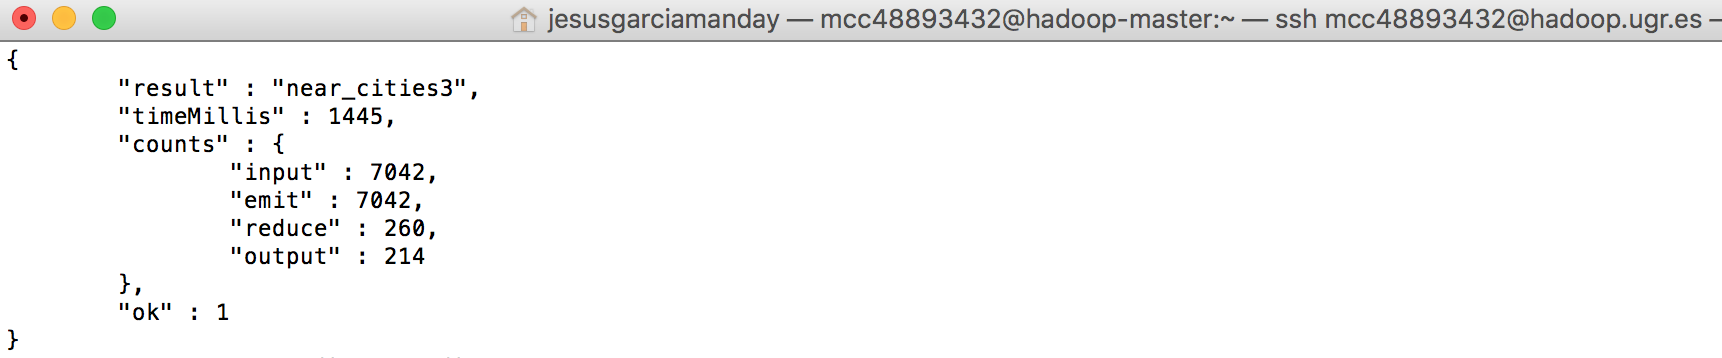
\includegraphics[width = 1.00\textwidth]{p3-img48}
 		\captionof{figure}{\label{fig:IPN}Visualizando los documentos (I).} 
	\end{center} 
\end{figure}

\begin{figure}[H]
	\begin{center}
 		\includegraphics[width = 1.00\textwidth]{p3-img49}
 		\captionof{figure}{\label{fig:IPN}Visualizando los documentos (II).} 
	\end{center} 
\end{figure}

\begin{figure}[H]
	\begin{center}
 		\includegraphics[width = 1.00\textwidth]{p3-img50}
 		\captionof{figure}{\label{fig:IPN}Visualizando los documentos (III).} 
	\end{center} 
\end{figure}

\begin{figure}[H]
	\begin{center}
 		\includegraphics[width = 1.00\textwidth]{p3-img51}
 		\captionof{figure}{\label{fig:IPN}Visualizando los documentos (IV).} 
	\end{center} 
\end{figure}

\begin{figure}[H]
	\begin{center}
 		\includegraphics[width = 1.00\textwidth]{p3-img52}
 		\captionof{figure}{\label{fig:IPN}Visualizando los documentos (V).} 
	\end{center} 
\end{figure}

 
\subsection{¿Cómo podríamos calcular la distancia media entre las ciudades de cada país?.}

\begin{figure}[H]
	\begin{center}
 		\includegraphics[width = 1.00\textwidth]{p3-img53}
 		\captionof{figure}{\label{fig:IPN}Visualizando los documentos (I).} 
	\end{center} 
\end{figure}

\begin{figure}[H]
	\begin{center}
 		\includegraphics[width = 1.00\textwidth]{p3-img54}
 		\captionof{figure}{\label{fig:IPN}Visualizando los documentos (II).} 
	\end{center} 
\end{figure}

\begin{figure}[H]
	\begin{center}
 		\includegraphics[width = 1.00\textwidth]{p3-img55}
 		\captionof{figure}{\label{fig:IPN}Visualizando los documentos (III).} 
	\end{center} 
\end{figure}

\begin{figure}[H]
	\begin{center}
 		\includegraphics[width = 1.00\textwidth]{p3-img56}
 		\captionof{figure}{\label{fig:IPN}Visualizando los documentos (IV).} 
	\end{center} 
\end{figure}

\begin{figure}[H]
	\begin{center}
 		\includegraphics[width = 1.00\textwidth]{p3-img57}
 		\captionof{figure}{\label{fig:IPN}Visualizando los documentos (V).} 
	\end{center} 
\end{figure}



\subsection{¿Mejoraría el rendimiento si creamos un índice?¿Sobre qué campo? Comprobadlo.}

\begin{figure}[H]
	\begin{center}
 		\includegraphics[width = 1.00\textwidth]{p3-img58}
 		\captionof{figure}{\label{fig:IPN}Visualizando los documentos.} 
	\end{center} 
\end{figure}

Se puede ver en la imagen como el rendimiento en tiempo no mejora, pero disminuye el número de entradas y salidas.




\end{document}